% Options for packages loaded elsewhere
\PassOptionsToPackage{unicode}{hyperref}
\PassOptionsToPackage{hyphens}{url}
%
\documentclass[
]{article}
\usepackage{amsmath,amssymb}
\usepackage{lmodern}
\usepackage{iftex}
\ifPDFTeX
  \usepackage[T1]{fontenc}
  \usepackage[utf8]{inputenc}
  \usepackage{textcomp} % provide euro and other symbols
\else % if luatex or xetex
  \usepackage{unicode-math}
  \defaultfontfeatures{Scale=MatchLowercase}
  \defaultfontfeatures[\rmfamily]{Ligatures=TeX,Scale=1}
\fi
% Use upquote if available, for straight quotes in verbatim environments
\IfFileExists{upquote.sty}{\usepackage{upquote}}{}
\IfFileExists{microtype.sty}{% use microtype if available
  \usepackage[]{microtype}
  \UseMicrotypeSet[protrusion]{basicmath} % disable protrusion for tt fonts
}{}
\makeatletter
\@ifundefined{KOMAClassName}{% if non-KOMA class
  \IfFileExists{parskip.sty}{%
    \usepackage{parskip}
  }{% else
    \setlength{\parindent}{0pt}
    \setlength{\parskip}{6pt plus 2pt minus 1pt}}
}{% if KOMA class
  \KOMAoptions{parskip=half}}
\makeatother
\usepackage{xcolor}
\IfFileExists{xurl.sty}{\usepackage{xurl}}{} % add URL line breaks if available
\IfFileExists{bookmark.sty}{\usepackage{bookmark}}{\usepackage{hyperref}}
\hypersetup{
  pdftitle={Relatório trabalho prático 2},
  pdfauthor={César A. Galvão 19/0011572; Gabriela Carneiro 18/0120816},
  hidelinks,
  pdfcreator={LaTeX via pandoc}}
\urlstyle{same} % disable monospaced font for URLs
\usepackage[margin=1in]{geometry}
\usepackage{color}
\usepackage{fancyvrb}
\newcommand{\VerbBar}{|}
\newcommand{\VERB}{\Verb[commandchars=\\\{\}]}
\DefineVerbatimEnvironment{Highlighting}{Verbatim}{commandchars=\\\{\}}
% Add ',fontsize=\small' for more characters per line
\usepackage{framed}
\definecolor{shadecolor}{RGB}{248,248,248}
\newenvironment{Shaded}{\begin{snugshade}}{\end{snugshade}}
\newcommand{\AlertTok}[1]{\textcolor[rgb]{0.94,0.16,0.16}{#1}}
\newcommand{\AnnotationTok}[1]{\textcolor[rgb]{0.56,0.35,0.01}{\textbf{\textit{#1}}}}
\newcommand{\AttributeTok}[1]{\textcolor[rgb]{0.77,0.63,0.00}{#1}}
\newcommand{\BaseNTok}[1]{\textcolor[rgb]{0.00,0.00,0.81}{#1}}
\newcommand{\BuiltInTok}[1]{#1}
\newcommand{\CharTok}[1]{\textcolor[rgb]{0.31,0.60,0.02}{#1}}
\newcommand{\CommentTok}[1]{\textcolor[rgb]{0.56,0.35,0.01}{\textit{#1}}}
\newcommand{\CommentVarTok}[1]{\textcolor[rgb]{0.56,0.35,0.01}{\textbf{\textit{#1}}}}
\newcommand{\ConstantTok}[1]{\textcolor[rgb]{0.00,0.00,0.00}{#1}}
\newcommand{\ControlFlowTok}[1]{\textcolor[rgb]{0.13,0.29,0.53}{\textbf{#1}}}
\newcommand{\DataTypeTok}[1]{\textcolor[rgb]{0.13,0.29,0.53}{#1}}
\newcommand{\DecValTok}[1]{\textcolor[rgb]{0.00,0.00,0.81}{#1}}
\newcommand{\DocumentationTok}[1]{\textcolor[rgb]{0.56,0.35,0.01}{\textbf{\textit{#1}}}}
\newcommand{\ErrorTok}[1]{\textcolor[rgb]{0.64,0.00,0.00}{\textbf{#1}}}
\newcommand{\ExtensionTok}[1]{#1}
\newcommand{\FloatTok}[1]{\textcolor[rgb]{0.00,0.00,0.81}{#1}}
\newcommand{\FunctionTok}[1]{\textcolor[rgb]{0.00,0.00,0.00}{#1}}
\newcommand{\ImportTok}[1]{#1}
\newcommand{\InformationTok}[1]{\textcolor[rgb]{0.56,0.35,0.01}{\textbf{\textit{#1}}}}
\newcommand{\KeywordTok}[1]{\textcolor[rgb]{0.13,0.29,0.53}{\textbf{#1}}}
\newcommand{\NormalTok}[1]{#1}
\newcommand{\OperatorTok}[1]{\textcolor[rgb]{0.81,0.36,0.00}{\textbf{#1}}}
\newcommand{\OtherTok}[1]{\textcolor[rgb]{0.56,0.35,0.01}{#1}}
\newcommand{\PreprocessorTok}[1]{\textcolor[rgb]{0.56,0.35,0.01}{\textit{#1}}}
\newcommand{\RegionMarkerTok}[1]{#1}
\newcommand{\SpecialCharTok}[1]{\textcolor[rgb]{0.00,0.00,0.00}{#1}}
\newcommand{\SpecialStringTok}[1]{\textcolor[rgb]{0.31,0.60,0.02}{#1}}
\newcommand{\StringTok}[1]{\textcolor[rgb]{0.31,0.60,0.02}{#1}}
\newcommand{\VariableTok}[1]{\textcolor[rgb]{0.00,0.00,0.00}{#1}}
\newcommand{\VerbatimStringTok}[1]{\textcolor[rgb]{0.31,0.60,0.02}{#1}}
\newcommand{\WarningTok}[1]{\textcolor[rgb]{0.56,0.35,0.01}{\textbf{\textit{#1}}}}
\usepackage{graphicx}
\makeatletter
\def\maxwidth{\ifdim\Gin@nat@width>\linewidth\linewidth\else\Gin@nat@width\fi}
\def\maxheight{\ifdim\Gin@nat@height>\textheight\textheight\else\Gin@nat@height\fi}
\makeatother
% Scale images if necessary, so that they will not overflow the page
% margins by default, and it is still possible to overwrite the defaults
% using explicit options in \includegraphics[width, height, ...]{}
\setkeys{Gin}{width=\maxwidth,height=\maxheight,keepaspectratio}
% Set default figure placement to htbp
\makeatletter
\def\fps@figure{htbp}
\makeatother
\setlength{\emergencystretch}{3em} % prevent overfull lines
\providecommand{\tightlist}{%
  \setlength{\itemsep}{0pt}\setlength{\parskip}{0pt}}
\setcounter{secnumdepth}{5}
\usepackage{helvet} \renewcommand\familydefault{\sfdefault}
\usepackage{booktabs}
\usepackage{longtable}
\usepackage{array}
\usepackage{multirow}
\usepackage{wrapfig}
\usepackage{float}
\usepackage{colortbl}
\usepackage{pdflscape}
\usepackage{tabu}
\usepackage{threeparttable}
\usepackage{threeparttablex}
\usepackage[normalem]{ulem}
\usepackage{makecell}
\usepackage{xcolor}
\ifLuaTeX
  \usepackage{selnolig}  % disable illegal ligatures
\fi

\title{Relatório trabalho prático 2}
\author{César A. Galvão 19/0011572 \and Gabriela Carneiro 18/0120816}
\date{18 de July de 2022}

\begin{document}
\maketitle

\newpage{}

{
\setcounter{tocdepth}{2}
\tableofcontents
}
\let\oldsection\section
\renewcommand\section{\clearpage\oldsection}

\begin{center} 

\textbf{Resumo} 

\end{center}

Nesta atividade foram implementadas em R métodos para geração de
variáveis aleatórias. Primeiramente foi criado um algoritmo para geração
de 200.000 números pseudo-aleatórios uniformemente distribuídos entre
(0, 1) pelo método congruencial linear. Este algoritmo foi então
utilizado para gerar variáveis aleatórias para diferentes distribuições
de probabilidade. A partir dos números pseudo-aleatórios, foram geradas
200.000 variáveis aleatórias de Poisson e 200.000 variáveis aleatórias
em distribuição exponencial, pelo método da transformação inversa. Para
gerar as 200.000 variáveis aleatórias em distribuição Normal foram
utilizados dois métodos: o método da rejeição e método polar. Todas as
variáveis geradas pelos métodos foram analisadas por meio de histogramas
e teste de aderência. Todos os testes confirmaram que as variáveis
geradas seguem as suas distribuições de referência. Por fim, foram
geradas tabelas de probabilidade para a distribuição normal pelos
métodos de Integração Monte Carlo, polar e da rejeição. Por meio das
simulações feitas, pode-se concluir que os métodos de geração das
variáveis aleatórias são eficientes e que dos métodos de geração
utilizados para a construção das tabelas de probabilidade, o polar é o
menos eficiente.\footnote{Todos os documentos desse relatório podem ser
  verificados no repositório
  \url{https://github.com/cesar-galvao/Estatistica-computacional}}

\hypertarget{introduuxe7uxe3o}{%
\section{Introdução}\label{introduuxe7uxe3o}}

Um número aleatório é um número gerado por meio de um processo cujo
resultado é probabilístico e, consequentemente, não pode ser reproduzido
de forma determinística. Um número aleatório pode ser gerado por meio de
experimentação, como em lançamentos de um dado, contagens de ocorrências
de raios gama, usando dígitos de pi, entre outros. No entanto, esses
métodos requerem grande esforço e tempo para serem utilizados.

Dessa forma, como alternativa, existem algoritmos que implementam
métodos para gerar números pseudo aleatórios. Um gerador de números
pseudo aleatórios é um algoritmo que cria sequências de números cujas
propriedades se assemelham às propriedades de números aleatórios, mas
que não podem ser classificados como aleatórios, pois as sequencias são
determinadas por um valor inicial, uma semente.

Dentre os métodos de geração de números pseudo aleatórios existe o
gerador linear congruencial. O gerador linear terá como output uma
distribuição uniforme. Depois disso, teoremas de estatística e
probabilidade serão utilizados para gerar outras variáveis aleatórias
correspondentes a outras distribuições, com base no gerador aleatório.

O gerador é definido pela relação de recorrência

\begin{align}
  X_{n+1} = \left( aX_n + c \right) \, \mod m 
\end{align}

em que \(a\) e \(m\) são inteiros positivos e \(\mod\) é o operador para
obtenção do resto da divisão.

A variável \(X\) retorna a sequência de números pseudo-aleatórios. Se
\(c = 0\), o gerador é chamado de gerador congruencial multiplicativo.
Se \(c \neq 0\), o gerador congruencial é chamado de gerador
congruencial misto.

Para gerar números aleatórios, um gerador linear congruencial será
desenvolvido. Esse gerador irá inicialmente ser utilizado para geração
de variáveis aleatórias uniformemente distribuídas no intervalo
\((0,1)\). A partir dessa função, serão geradas variáveis aleatórias nas
distribuições de Poisson, exponencial, e normal padrão.

\hypertarget{muxe9todo}{%
\section{Método}\label{muxe9todo}}

\hypertarget{variuxe1vel-aleatuxf3ria-uniforme}{%
\subsection{Variável aleatória
uniforme}\label{variuxe1vel-aleatuxf3ria-uniforme}}

A geração da variável aleatória uniforme segue o seguinte algoritmo:

\begin{enumerate}
\def\labelenumi{\arabic{enumi}.}
\tightlist
\item
  As constantes \(a\) e \(m\) são definidas. Aqui, foram utilizados
  \(a = 16.807\) e \(m = 2^{31}-1\);
\item
  Uma semente aleatória é obtida utilizando o relógio do sistema pela
  função \texttt{Sys.time()};
\item
  A semente é redefinida \(y_{i+1} = (a \cdot y_i) \mod m\);
\item
  O número pertencente a \(U(0,1)\) é gerado \(x_i = y_{i+1}/m\).
\end{enumerate}

\hypertarget{variuxe1vel-aleatuxf3ria-poisson}{%
\subsection{Variável aleatória
Poisson}\label{variuxe1vel-aleatuxf3ria-poisson}}

O algoritmo gera uma variável aleatória que segue a distribuição Poisson
com média \(\lambda\). Primeiramente ele gera um número aleatório
uniformemente distribuído \(U\) e verifica \(U < e^{-\lambda} = p_0\).
Se for menor, o algoritmo assume \(X = 0\). Caso contrário, ele itera o
laço e verifica novamente novamente a condição, mas agora para a
proposição \(U < p_0 + p_1\). Se o valor for menor, o algoritmo atribui
\(X = 1\).

O algoritmo implementado verifica sucessivamente se o valor da Poisson é
zero, em seguida verifica se o valor é 1, então 2 e assim por diante.
Dessa forma, o número de comparações necessários será uma unidade maior
que o valor da Poisson (1 + \(\lambda\)). Para valores pequenos de
\(\lambda\) o programa é eficiente, mas quando \(\lambda\) assume
valores muito grandes esse algoritmo não é o mais otimizado. O ideal é
escolher valores mais próximos de lambda para iniciar a verificação do
laço. A implementação escolhida foi a primeira, não otimizada.

\hypertarget{variuxe1vel-aleatuxf3ria-exponencial}{%
\subsection{Variável aleatória
exponencial}\label{variuxe1vel-aleatuxf3ria-exponencial}}

Para gerar variáveis na distribuição exponencial, o método implementado
foi o da transformação inversa.

Supondo que \(X\) é uma variável aleatória com distribuição exponencial
de \(\lambda = 1\), sua função de distribuição pode ser expressa por

\begin{align}
  F(x) = 1 - e^{-x}
\end{align}

Se, \(x = F^{-1}(u)\), então,

\begin{align}
  u = F(x) = 1 - e^{-x} \longrightarrow 1 - u = e^{-x}
\end{align}

Aplicando o logaritmo, tem-se \(x = - log(1 - u)\). Dessa forma, podemos
gerar \(X\) por meio de um número aleatório distribuído uniformemente e
definindo \(X = F^{-1}(U) = - \log(1 - U)\).

Uma pequena economia de tempo pode ser obtida observando que \(1 - U\)
também é uniforme em \((0, 1)\) e assim \(-\log(1 - U)\) tem a mesma
distribuição que \(-\log U\). Ou seja, o logaritmo negativo de um número
aleatório é distribuído exponencialmente com \(\lambda = 1\).

Além disso, observa-se que se \(X\) é exponencial com média 1, então,
para qualquer constante \(c\), \(cX\) é exponencial com média \(c\).
Portanto, uma variável aleatória exponencial \(X\) com parâmetro
\(\lambda\) (média \(1/\lambda\)) pode ser gerada por meio de um número
aleatório \(U\) e definindo:

\begin{align}
  X = \frac{-1}{\lambda} \cdot \log U
\end{align}

\newpage

\hypertarget{variuxe1vel-aleatuxf3ria-normal}{%
\subsection{Variável aleatória
Normal}\label{variuxe1vel-aleatuxf3ria-normal}}

\hypertarget{muxe9todo-polar}{%
\subsubsection{Método polar}\label{muxe9todo-polar}}

O método polar segue a abordagem abaixo para gerar um par de normais
padrão independentes:

\begin{enumerate}
\def\labelenumi{\arabic{enumi}.}
\tightlist
\item
  Gerar números pseudo aleatórios uniformente distribuídos, \(U_1\) e
  \(U_2\);
\item
  Gerar
  \(V_1 = 2 U_1 - 1, \, \, V_2 = 2 U_2 - 1, \,\, S = V_1^2 + V_2^2\);
\item
  Se \(S > 1\), retornar ao passo 1;
\item
  Retornar as variáveis independentes com distribuição normal padrão.
\end{enumerate}

\begin{align}
  X = \sqrt{\frac{-2 \log S}{S}}V_1, \quad Y = \sqrt{\frac{-2 \log S}{S}}V_2
\end{align}

\hypertarget{muxe9todo-da-rejeiuxe7uxe3o}{%
\subsubsection{Método da rejeição}\label{muxe9todo-da-rejeiuxe7uxe3o}}

O método da rejeição gera valores de uma distribuição \(X\) com função
de densidade \(f(x)\) a partir de uma distribuição de partida \(Y\) com
densidade de probabilidade \(g(x)\). A ideia é que se pode gerar um
valor de \(X\) por meio de \(Y\) aceitando ou não o valor de \(Y\) com
probabilidade \(\frac{f(y)}{c \, g(y)}\). As comparações são repetidas
\(Y\) até que um valor seja aceito. Especificamente, seja \(c\) uma
constante tal que \(f(y)/g(y) \leq c\), para todo \(y\). Dessa forma, a
técnica a seguir gera uma variável aleatória com densidade f:

\begin{enumerate}
\def\labelenumi{\arabic{enumi}.}
\tightlist
\item
  Gerar \(Y\) tendo densidade \(g\);
\item
  Gerar um número pseudo-aleatório \(U\);
\item
  Se \(U \leq \frac{f(y)}{c\, g(y)}\), assumir \(X = Y\). Caso
  contrário, retornar para passo 1.
\end{enumerate}

Com base nisso, pode-se afirmar que a variável aleatória gerada pelo
método de rejeição tem densidade \(f\) e que o número de iterações do
algoritmo que são necessárias é um número que segue uma distribuição
geométrica com média \(c\).

O histograma mostra que as variáveis aleatórias geradas pelo método
aparentemente têm uma tendencia normal, apesar de apresentar uma queda
em torno do zero. Assim como as distribuições anteriores, o fato de o
gerador do número pseudo-aleatório uniforme não ter se comportado como o
esperado nas extremidades pode ter afetado a geração das variáveis
aleatórias normalmente distribuídas.

\hypertarget{resultados}{%
\section{Resultados}\label{resultados}}

A seguir são expostas duas comparações para avaliação da qualidade de
cada um dos algoritmos utilizados: a primeira é gráfica e expõe
histogramas das distribuições geradas e a linha correspondente à
distribuição teórica. A segunda é a realização de testes de aderência
qui-quadrado, os quais foram realizados comparando os quartis das
distribuições empíricas com as distribuições hipotéticas.

Para os testes de aderência, as hipóteses utilizadas são as mesmas em
todos os casos:

\begin{align}
  \begin{cases}
    H_0: \text{não existe diferença significativa entre os valores observados e os esperados}; \\
    H_a: \text{existe diferença significativa entre os valores observados e os esperados};
  \end{cases}
\end{align}

Além disso, todas as amostras têm tamanho \(n = 200.000\).

\hypertarget{uniforme}{%
\subsection{Uniforme}\label{uniforme}}

A amostra gerada para a distribuição uniforme se aproxima graficamente
de sua função densidade teórica. Exceções podem ser observadas nos
valores extremos da amostra e os motivos para isso, pelo menos
graficamente, podem ser dois:

\begin{enumerate}
\def\labelenumi{\arabic{enumi}.}
\tightlist
\item
  De fato o algoritmo utilizado gera precariamente valores nas
  extremidades da distribuição; ou\\
\item
  O histograma gerado utiliza valores acima e abaixo dos centros das
  barras para projetar a altura das barras. Como valores abaixo de 0 e
  acima de 1 não existem, suas barras são mais curtas.
\end{enumerate}

\begin{figure}

{\centering 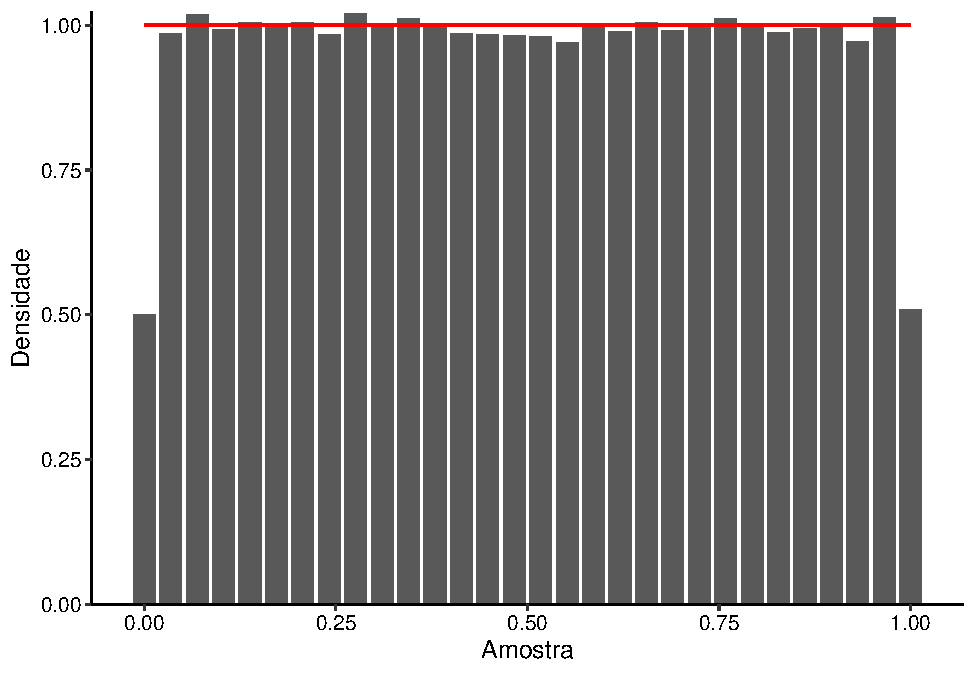
\includegraphics[width=0.7\linewidth]{relatorio_tp2_files/figure-latex/resultados-unif-1} 

}

\caption{Histograma da amostra de v.a. uniforme com linha da f.d.p. uniforme}\label{fig:resultados-unif}
\end{figure}

Ao realizar o teste de aderência, obtém-se p-valor igual a 1,
corroborando a maior chance de o tópico 2 ser o motivo para as barras
mais curtas nas extremidades. O teste indica portanto que, utilizando a
distribuição dos quartis da amostra, não seria possível diferenciá-la de
uma variável aleatória com distribuição uniforme teórica.

\hypertarget{poisson}{%
\subsection{Poisson}\label{poisson}}

O gráfico gerado para a v.a. Poisson suscita as mesmas dúvidas quanto à
altura das barras. Nota-se que as barras estão abaixo dos pontos
teóricos enquanto estão também deslocados em relação aos centros das
barras.

\begin{figure}

{\centering 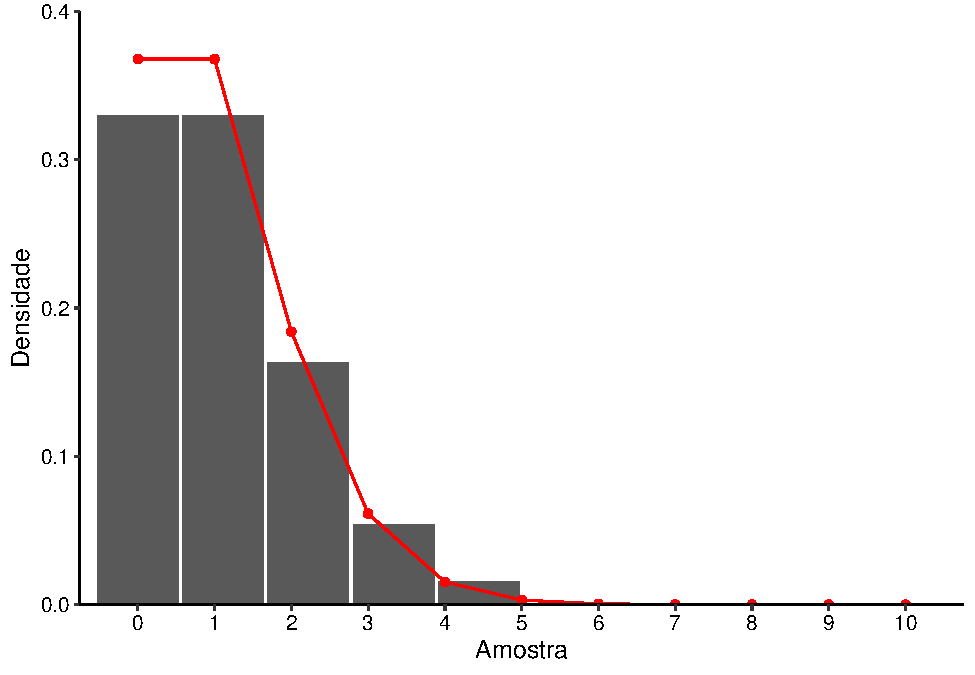
\includegraphics[width=0.7\linewidth]{relatorio_tp2_files/figure-latex/resultados-pois-1} 

}

\caption{Histograma da amostra de v.a. Poisson com linha da f.p. Poisson}\label{fig:resultados-pois}
\end{figure}

O teste de aderência para a distribuição indica p-valor muito próximo de
1, o que sugere novamente uma dificuldade de composição do gráfico e a
impossibilidade de diferenciar a distribuição da amostra da distribuição
teórica.

\pagebreak

\hypertarget{exponencial}{%
\subsection{Exponencial}\label{exponencial}}

A amostra gerada para a distribuição exponencial também parece estar
próxima da distribuição teórica, a menos da barra inicial correspondente
a valores próximos a zero.

\begin{figure}

{\centering 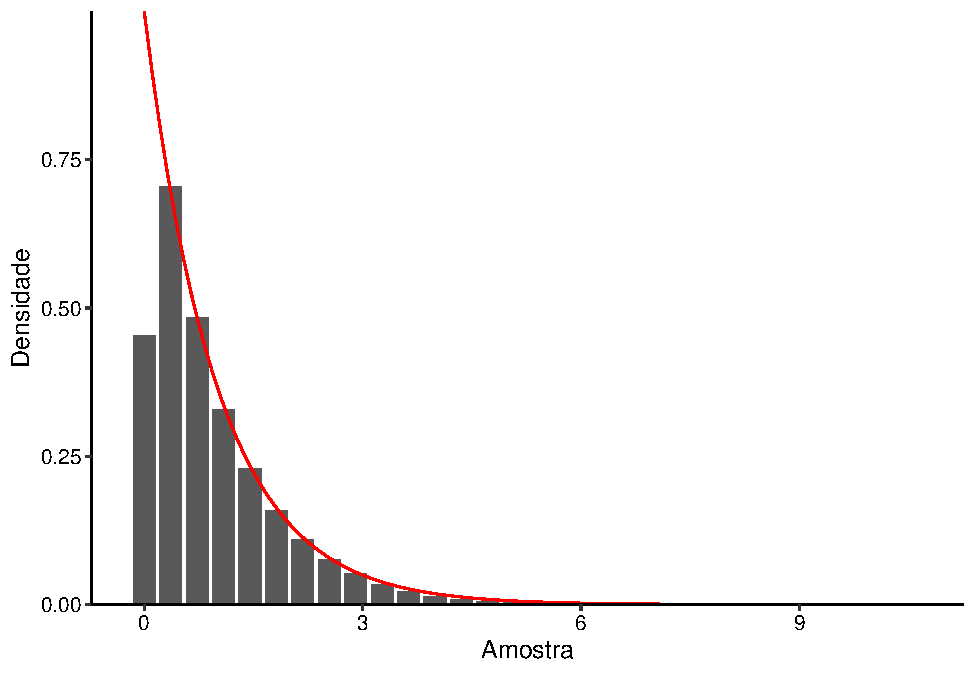
\includegraphics[width=0.7\linewidth]{relatorio_tp2_files/figure-latex/resultados-exp-1} 

}

\caption{Histograma da amostra de v.a. exponencial com linha da f.d.p. exponencial}\label{fig:resultados-exp}
\end{figure}

Novamente o teste de aderência é realizado com p-valor 1, sugerindo a
impossibilidade de diferenciação da distribuição da amostra em relação à
distribuição teórica.

\newpage

\hypertarget{normal}{%
\subsection{Normal}\label{normal}}

O histograma mostra que as variáveis aleatórias geradas pelo método
aparentemente têm uma tendencia normal, apesar de apresentar uma queda
em torno do zero. Assim como as distribuições anteriores, o fato de o
gerador do número pseudo-aleatório uniforme não ter se comportado como o
esperado nas extremidades pode ter afetado a geração das variáveis
aleatórias normalmente distribuídas.

\begin{figure}

{\centering 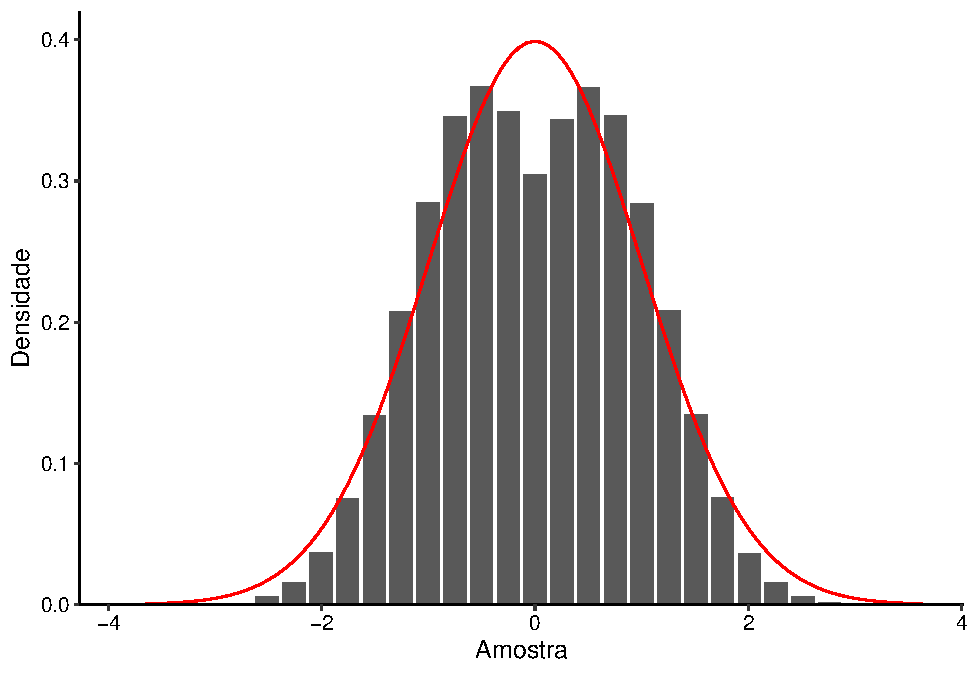
\includegraphics[width=0.7\linewidth]{relatorio_tp2_files/figure-latex/resultados-norm-rej-1} 

}

\caption{Histograma da amostra de v.a. normal, método rejeição, com linha da f.d.p. normal}\label{fig:resultados-norm-rej}
\end{figure}

\pagebreak

Conforme histograma a seguir, tanto X quanto Y gerados pelo método polar
seguem distribuição normal com médias centradas em zero.

\begin{figure}

{\centering 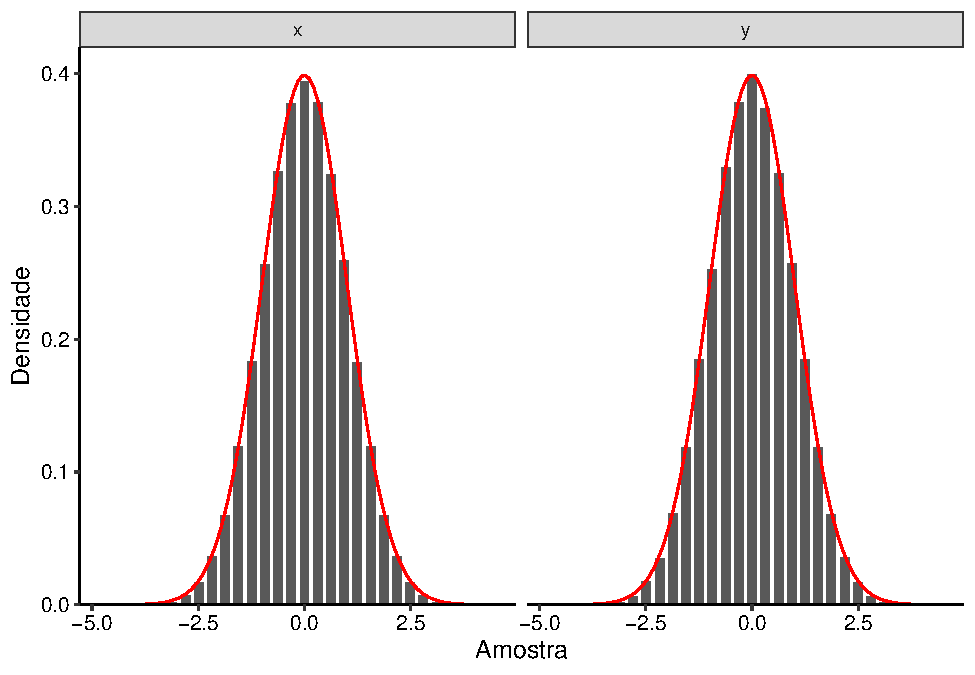
\includegraphics[width=0.7\linewidth]{relatorio_tp2_files/figure-latex/resultados-norm-pol-1} 

}

\caption{Histograma da amostra de v.a. normal, método polar, com linha da f.d.p. normal}\label{fig:resultados-norm-pol}
\end{figure}

\hypertarget{tabelas-normal-estimadas}{%
\section{Tabelas Normal estimadas}\label{tabelas-normal-estimadas}}

As estimações a seguir consideram a probabilidade acumulada de
\((-\infty, b]\). É esperado que os valores variem de 0.5 a 1, no
entanto as aproximações realizadas pelos métodos de Integração de Monte
Carlo e os demais utilizados para geração de amostras normais estão
suscetíveis a erros aleatórios. Observa-se nas tabelas a seguir esses
erros de estimação quando se atinge, antes do valor máximo dos quantis
disponíveis, \(p=1\) ou \(p < 1\).

\hypertarget{tabela-integrauxe7uxe3o-monte-carlo}{%
\subsection{Tabela Integração Monte
Carlo}\label{tabela-integrauxe7uxe3o-monte-carlo}}

\begin{longtable}[l]{lcccccccccc}
\toprule
  & 0 & 0.01 & 0.02 & 0.03 & 0.04 & 0.05 & 0.06 & 0.07 & 0.08 & 0.09\\
\midrule
\endfirsthead
\multicolumn{11}{@{}l}{\textit{(continued)}}\\
\toprule
  & 0 & 0.01 & 0.02 & 0.03 & 0.04 & 0.05 & 0.06 & 0.07 & 0.08 & 0.09\\
\midrule
\endhead

\endfoot
\bottomrule
\endlastfoot
\cellcolor{gray!15}{0} & \cellcolor{gray!15}{0.5000} & \cellcolor{gray!15}{0.5040} & \cellcolor{gray!15}{0.5080} & \cellcolor{gray!15}{0.5120} & \cellcolor{gray!15}{0.5160} & \cellcolor{gray!15}{0.5199} & \cellcolor{gray!15}{0.5239} & \cellcolor{gray!15}{0.5279} & \cellcolor{gray!15}{0.5319} & \cellcolor{gray!15}{0.5359}\\
0.1 & 0.5398 & 0.5438 & 0.5478 & 0.5517 & 0.5557 & 0.5596 & 0.5636 & 0.5675 & 0.5714 & 0.5753\\
\cellcolor{gray!15}{0.2} & \cellcolor{gray!15}{0.5793} & \cellcolor{gray!15}{0.5832} & \cellcolor{gray!15}{0.5871} & \cellcolor{gray!15}{0.5910} & \cellcolor{gray!15}{0.5948} & \cellcolor{gray!15}{0.5987} & \cellcolor{gray!15}{0.6026} & \cellcolor{gray!15}{0.6064} & \cellcolor{gray!15}{0.6103} & \cellcolor{gray!15}{0.6141}\\
0.3 & 0.6179 & 0.6217 & 0.6255 & 0.6293 & 0.6331 & 0.6368 & 0.6406 & 0.6443 & 0.6480 & 0.6517\\
\cellcolor{gray!15}{0.4} & \cellcolor{gray!15}{0.6554} & \cellcolor{gray!15}{0.6591} & \cellcolor{gray!15}{0.6628} & \cellcolor{gray!15}{0.6664} & \cellcolor{gray!15}{0.6700} & \cellcolor{gray!15}{0.6737} & \cellcolor{gray!15}{0.6773} & \cellcolor{gray!15}{0.6808} & \cellcolor{gray!15}{0.6844} & \cellcolor{gray!15}{0.6879}\\
0.5 & 0.6915 & 0.6950 & 0.6985 & 0.7020 & 0.7054 & 0.7089 & 0.7123 & 0.7157 & 0.7191 & 0.7224\\
\cellcolor{gray!15}{0.6} & \cellcolor{gray!15}{0.7258} & \cellcolor{gray!15}{0.7291} & \cellcolor{gray!15}{0.7324} & \cellcolor{gray!15}{0.7357} & \cellcolor{gray!15}{0.7389} & \cellcolor{gray!15}{0.7422} & \cellcolor{gray!15}{0.7454} & \cellcolor{gray!15}{0.7486} & \cellcolor{gray!15}{0.7518} & \cellcolor{gray!15}{0.7549}\\
0.7 & 0.7581 & 0.7612 & 0.7643 & 0.7673 & 0.7704 & 0.7734 & 0.7764 & 0.7794 & 0.7823 & 0.7853\\
\cellcolor{gray!15}{0.8} & \cellcolor{gray!15}{0.7882} & \cellcolor{gray!15}{0.7911} & \cellcolor{gray!15}{0.7939} & \cellcolor{gray!15}{0.7968} & \cellcolor{gray!15}{0.7996} & \cellcolor{gray!15}{0.8024} & \cellcolor{gray!15}{0.8052} & \cellcolor{gray!15}{0.8079} & \cellcolor{gray!15}{0.8106} & \cellcolor{gray!15}{0.8133}\\
0.9 & 0.8160 & 0.8186 & 0.8213 & 0.8239 & 0.8265 & 0.8290 & 0.8315 & 0.8340 & 0.8365 & 0.8390\\
\cellcolor{gray!15}{1} & \cellcolor{gray!15}{0.8414} & \cellcolor{gray!15}{0.8438} & \cellcolor{gray!15}{0.8462} & \cellcolor{gray!15}{0.8486} & \cellcolor{gray!15}{0.8509} & \cellcolor{gray!15}{0.8532} & \cellcolor{gray!15}{0.8555} & \cellcolor{gray!15}{0.8578} & \cellcolor{gray!15}{0.8600} & \cellcolor{gray!15}{0.8622}\\
1.1 & 0.8644 & 0.8666 & 0.8687 & 0.8708 & 0.8729 & 0.8750 & 0.8771 & 0.8791 & 0.8811 & 0.8831\\
\cellcolor{gray!15}{1.2} & \cellcolor{gray!15}{0.8850} & \cellcolor{gray!15}{0.8869} & \cellcolor{gray!15}{0.8889} & \cellcolor{gray!15}{0.8907} & \cellcolor{gray!15}{0.8926} & \cellcolor{gray!15}{0.8944} & \cellcolor{gray!15}{0.8963} & \cellcolor{gray!15}{0.8980} & \cellcolor{gray!15}{0.8998} & \cellcolor{gray!15}{0.9016}\\
1.3 & 0.9033 & 0.9050 & 0.9067 & 0.9083 & 0.9100 & 0.9116 & 0.9132 & 0.9147 & 0.9163 & 0.9178\\
\cellcolor{gray!15}{1.4} & \cellcolor{gray!15}{0.9193} & \cellcolor{gray!15}{0.9208} & \cellcolor{gray!15}{0.9223} & \cellcolor{gray!15}{0.9237} & \cellcolor{gray!15}{0.9251} & \cellcolor{gray!15}{0.9266} & \cellcolor{gray!15}{0.9279} & \cellcolor{gray!15}{0.9293} & \cellcolor{gray!15}{0.9306} & \cellcolor{gray!15}{0.9320}\\
1.5 & 0.9333 & 0.9345 & 0.9358 & 0.9371 & 0.9383 & 0.9395 & 0.9407 & 0.9419 & 0.9430 & 0.9441\\
\cellcolor{gray!15}{1.6} & \cellcolor{gray!15}{0.9453} & \cellcolor{gray!15}{0.9463} & \cellcolor{gray!15}{0.9474} & \cellcolor{gray!15}{0.9485} & \cellcolor{gray!15}{0.9495} & \cellcolor{gray!15}{0.9506} & \cellcolor{gray!15}{0.9516} & \cellcolor{gray!15}{0.9526} & \cellcolor{gray!15}{0.9535} & \cellcolor{gray!15}{0.9545}\\
1.7 & 0.9555 & 0.9564 & 0.9573 & 0.9582 & 0.9591 & 0.9599 & 0.9608 & 0.9616 & 0.9624 & 0.9633\\
\cellcolor{gray!15}{1.8} & \cellcolor{gray!15}{0.9640} & \cellcolor{gray!15}{0.9648} & \cellcolor{gray!15}{0.9656} & \cellcolor{gray!15}{0.9663} & \cellcolor{gray!15}{0.9671} & \cellcolor{gray!15}{0.9678} & \cellcolor{gray!15}{0.9685} & \cellcolor{gray!15}{0.9692} & \cellcolor{gray!15}{0.9699} & \cellcolor{gray!15}{0.9706}\\
1.9 & 0.9712 & 0.9719 & 0.9725 & 0.9731 & 0.9737 & 0.9743 & 0.9749 & 0.9755 & 0.9760 & 0.9766\\
\cellcolor{gray!15}{2} & \cellcolor{gray!15}{0.9771} & \cellcolor{gray!15}{0.9776} & \cellcolor{gray!15}{0.9781} & \cellcolor{gray!15}{0.9787} & \cellcolor{gray!15}{0.9792} & \cellcolor{gray!15}{0.9796} & \cellcolor{gray!15}{0.9801} & \cellcolor{gray!15}{0.9806} & \cellcolor{gray!15}{0.9810} & \cellcolor{gray!15}{0.9815}\\
2.1 & 0.9819 & 0.9823 & 0.9828 & 0.9832 & 0.9836 & 0.9840 & 0.9843 & 0.9847 & 0.9851 & 0.9854\\
\cellcolor{gray!15}{2.2} & \cellcolor{gray!15}{0.9858} & \cellcolor{gray!15}{0.9861} & \cellcolor{gray!15}{0.9865} & \cellcolor{gray!15}{0.9868} & \cellcolor{gray!15}{0.9871} & \cellcolor{gray!15}{0.9874} & \cellcolor{gray!15}{0.9877} & \cellcolor{gray!15}{0.9880} & \cellcolor{gray!15}{0.9883} & \cellcolor{gray!15}{0.9886}\\
2.3 & 0.9889 & 0.9891 & 0.9894 & 0.9896 & 0.9899 & 0.9901 & 0.9904 & 0.9906 & 0.9908 & 0.9911\\
\cellcolor{gray!15}{2.4} & \cellcolor{gray!15}{0.9913} & \cellcolor{gray!15}{0.9915} & \cellcolor{gray!15}{0.9917} & \cellcolor{gray!15}{0.9919} & \cellcolor{gray!15}{0.9921} & \cellcolor{gray!15}{0.9923} & \cellcolor{gray!15}{0.9924} & \cellcolor{gray!15}{0.9926} & \cellcolor{gray!15}{0.9928} & \cellcolor{gray!15}{0.9930}\\
2.5 & 0.9931 & 0.9933 & 0.9934 & 0.9936 & 0.9937 & 0.9939 & 0.9940 & 0.9942 & 0.9943 & 0.9944\\
\cellcolor{gray!15}{2.6} & \cellcolor{gray!15}{0.9945} & \cellcolor{gray!15}{0.9947} & \cellcolor{gray!15}{0.9948} & \cellcolor{gray!15}{0.9949} & \cellcolor{gray!15}{0.9950} & \cellcolor{gray!15}{0.9951} & \cellcolor{gray!15}{0.9952} & \cellcolor{gray!15}{0.9953} & \cellcolor{gray!15}{0.9954} & \cellcolor{gray!15}{0.9955}\\
2.7 & 0.9956 & 0.9957 & 0.9958 & 0.9959 & 0.9959 & 0.9960 & 0.9961 & 0.9962 & 0.9962 & 0.9963\\
\cellcolor{gray!15}{2.8} & \cellcolor{gray!15}{0.9964} & \cellcolor{gray!15}{0.9964} & \cellcolor{gray!15}{0.9965} & \cellcolor{gray!15}{0.9965} & \cellcolor{gray!15}{0.9966} & \cellcolor{gray!15}{0.9966} & \cellcolor{gray!15}{0.9967} & \cellcolor{gray!15}{0.9967} & \cellcolor{gray!15}{0.9968} & \cellcolor{gray!15}{0.9968}\\
2.9 & 0.9969 & 0.9969 & 0.9970 & 0.9970 & 0.9970 & 0.9971 & 0.9971 & 0.9971 & 0.9972 & 0.9972\\
\cellcolor{gray!15}{3} & \cellcolor{gray!15}{0.9972} & \cellcolor{gray!15}{0.9973} & \cellcolor{gray!15}{0.9973} & \cellcolor{gray!15}{0.9973} & \cellcolor{gray!15}{0.9973} & \cellcolor{gray!15}{0.9974} & \cellcolor{gray!15}{0.9974} & \cellcolor{gray!15}{0.9974} & \cellcolor{gray!15}{0.9974} & \cellcolor{gray!15}{0.9974}\\
3.1 & 0.9975 & 0.9975 & 0.9975 & 0.9975 & 0.9975 & 0.9975 & 0.9975 & 0.9975 & 0.9975 & 0.9976\\
\cellcolor{gray!15}{3.2} & \cellcolor{gray!15}{0.9976} & \cellcolor{gray!15}{0.9976} & \cellcolor{gray!15}{0.9976} & \cellcolor{gray!15}{0.9976} & \cellcolor{gray!15}{0.9976} & \cellcolor{gray!15}{0.9976} & \cellcolor{gray!15}{0.9976} & \cellcolor{gray!15}{0.9976} & \cellcolor{gray!15}{0.9976} & \cellcolor{gray!15}{0.9976}\\
3.3 & 0.9976 & 0.9976 & 0.9976 & 0.9976 & 0.9976 & 0.9976 & 0.9976 & 0.9976 & 0.9976 & 0.9976\\
\cellcolor{gray!15}{3.4} & \cellcolor{gray!15}{0.9976} & \cellcolor{gray!15}{0.9976} & \cellcolor{gray!15}{0.9976} & \cellcolor{gray!15}{0.9975} & \cellcolor{gray!15}{0.9975} & \cellcolor{gray!15}{0.9975} & \cellcolor{gray!15}{0.9975} & \cellcolor{gray!15}{0.9975} & \cellcolor{gray!15}{0.9975} & \cellcolor{gray!15}{0.9975}\\
3.5 & 0.9975 & 0.9975 & 0.9975 & 0.9975 & 0.9975 & 0.9974 & 0.9974 & 0.9974 & 0.9974 & 0.9974\\
\cellcolor{gray!15}{3.6} & \cellcolor{gray!15}{0.9974} & \cellcolor{gray!15}{0.9974} & \cellcolor{gray!15}{0.9974} & \cellcolor{gray!15}{0.9974} & \cellcolor{gray!15}{0.9973} & \cellcolor{gray!15}{0.9973} & \cellcolor{gray!15}{0.9973} & \cellcolor{gray!15}{0.9973} & \cellcolor{gray!15}{0.9973} & \cellcolor{gray!15}{0.9973}\\
3.7 & 0.9973 & 0.9973 & 0.9972 & 0.9972 & 0.9972 & 0.9972 & 0.9972 & 0.9972 & 0.9972 & 0.9971\\
\cellcolor{gray!15}{3.8} & \cellcolor{gray!15}{0.9971} & \cellcolor{gray!15}{0.9971} & \cellcolor{gray!15}{0.9971} & \cellcolor{gray!15}{0.9971} & \cellcolor{gray!15}{0.9971} & \cellcolor{gray!15}{0.9971} & \cellcolor{gray!15}{0.9970} & \cellcolor{gray!15}{0.9970} & \cellcolor{gray!15}{0.9970} & \cellcolor{gray!15}{0.9970}\\
3.9 & 0.9970 & 0.9970 & 0.9970 & 0.9969 & 0.9969 & 0.9969 & 0.9969 & 0.9969 & 0.9969 & 0.9968\\*
\end{longtable}

\newpage

\hypertarget{tabela-estimada-pelo-muxe9todo-polar}{%
\subsection{Tabela estimada pelo método
polar}\label{tabela-estimada-pelo-muxe9todo-polar}}

\begin{longtable}[l]{lcccccccccc}
\toprule
  & 0 & 0.01 & 0.02 & 0.03 & 0.04 & 0.05 & 0.06 & 0.07 & 0.08 & 0.09\\
\midrule
\endfirsthead
\multicolumn{11}{@{}l}{\textit{(continued)}}\\
\toprule
  & 0 & 0.01 & 0.02 & 0.03 & 0.04 & 0.05 & 0.06 & 0.07 & 0.08 & 0.09\\
\midrule
\endhead

\endfoot
\bottomrule
\endlastfoot
\cellcolor{gray!15}{0} & \cellcolor{gray!15}{0.5000} & \cellcolor{gray!15}{0.5039} & \cellcolor{gray!15}{0.5075} & \cellcolor{gray!15}{0.5115} & \cellcolor{gray!15}{0.5156} & \cellcolor{gray!15}{0.5195} & \cellcolor{gray!15}{0.5235} & \cellcolor{gray!15}{0.5277} & \cellcolor{gray!15}{0.5319} & \cellcolor{gray!15}{0.5359}\\
0.1 & 0.5399 & 0.5438 & 0.5478 & 0.5517 & 0.5555 & 0.5592 & 0.5631 & 0.5669 & 0.5708 & 0.5749\\
\cellcolor{gray!15}{0.2} & \cellcolor{gray!15}{0.5789} & \cellcolor{gray!15}{0.5830} & \cellcolor{gray!15}{0.5867} & \cellcolor{gray!15}{0.5906} & \cellcolor{gray!15}{0.5944} & \cellcolor{gray!15}{0.5983} & \cellcolor{gray!15}{0.6023} & \cellcolor{gray!15}{0.6061} & \cellcolor{gray!15}{0.6102} & \cellcolor{gray!15}{0.6140}\\
0.3 & 0.6178 & 0.6217 & 0.6255 & 0.6292 & 0.6330 & 0.6367 & 0.6405 & 0.6443 & 0.6477 & 0.6513\\
\cellcolor{gray!15}{0.4} & \cellcolor{gray!15}{0.6549} & \cellcolor{gray!15}{0.6585} & \cellcolor{gray!15}{0.6622} & \cellcolor{gray!15}{0.6661} & \cellcolor{gray!15}{0.6699} & \cellcolor{gray!15}{0.6736} & \cellcolor{gray!15}{0.6773} & \cellcolor{gray!15}{0.6808} & \cellcolor{gray!15}{0.6842} & \cellcolor{gray!15}{0.6879}\\
0.5 & 0.6914 & 0.6949 & 0.6984 & 0.7016 & 0.7051 & 0.7084 & 0.7119 & 0.7154 & 0.7188 & 0.7221\\
\cellcolor{gray!15}{0.6} & \cellcolor{gray!15}{0.7254} & \cellcolor{gray!15}{0.7288} & \cellcolor{gray!15}{0.7320} & \cellcolor{gray!15}{0.7353} & \cellcolor{gray!15}{0.7387} & \cellcolor{gray!15}{0.7418} & \cellcolor{gray!15}{0.7449} & \cellcolor{gray!15}{0.7480} & \cellcolor{gray!15}{0.7511} & \cellcolor{gray!15}{0.7543}\\
0.7 & 0.7574 & 0.7605 & 0.7634 & 0.7664 & 0.7694 & 0.7723 & 0.7754 & 0.7784 & 0.7815 & 0.7844\\
\cellcolor{gray!15}{0.8} & \cellcolor{gray!15}{0.7875} & \cellcolor{gray!15}{0.7903} & \cellcolor{gray!15}{0.7931} & \cellcolor{gray!15}{0.7959} & \cellcolor{gray!15}{0.7988} & \cellcolor{gray!15}{0.8015} & \cellcolor{gray!15}{0.8044} & \cellcolor{gray!15}{0.8072} & \cellcolor{gray!15}{0.8100} & \cellcolor{gray!15}{0.8129}\\
0.9 & 0.8155 & 0.8183 & 0.8209 & 0.8234 & 0.8262 & 0.8288 & 0.8314 & 0.8338 & 0.8361 & 0.8386\\
\cellcolor{gray!15}{1} & \cellcolor{gray!15}{0.8409} & \cellcolor{gray!15}{0.8434} & \cellcolor{gray!15}{0.8458} & \cellcolor{gray!15}{0.8481} & \cellcolor{gray!15}{0.8504} & \cellcolor{gray!15}{0.8528} & \cellcolor{gray!15}{0.8553} & \cellcolor{gray!15}{0.8577} & \cellcolor{gray!15}{0.8601} & \cellcolor{gray!15}{0.8623}\\
1.1 & 0.8645 & 0.8668 & 0.8689 & 0.8710 & 0.8732 & 0.8753 & 0.8773 & 0.8794 & 0.8814 & 0.8834\\
\cellcolor{gray!15}{1.2} & \cellcolor{gray!15}{0.8854} & \cellcolor{gray!15}{0.8874} & \cellcolor{gray!15}{0.8894} & \cellcolor{gray!15}{0.8913} & \cellcolor{gray!15}{0.8933} & \cellcolor{gray!15}{0.8950} & \cellcolor{gray!15}{0.8969} & \cellcolor{gray!15}{0.8987} & \cellcolor{gray!15}{0.9004} & \cellcolor{gray!15}{0.9020}\\
1.3 & 0.9038 & 0.9055 & 0.9071 & 0.9088 & 0.9105 & 0.9119 & 0.9134 & 0.9148 & 0.9163 & 0.9179\\
\cellcolor{gray!15}{1.4} & \cellcolor{gray!15}{0.9193} & \cellcolor{gray!15}{0.9207} & \cellcolor{gray!15}{0.9222} & \cellcolor{gray!15}{0.9238} & \cellcolor{gray!15}{0.9252} & \cellcolor{gray!15}{0.9265} & \cellcolor{gray!15}{0.9278} & \cellcolor{gray!15}{0.9294} & \cellcolor{gray!15}{0.9307} & \cellcolor{gray!15}{0.9320}\\
1.5 & 0.9332 & 0.9345 & 0.9358 & 0.9372 & 0.9384 & 0.9396 & 0.9408 & 0.9419 & 0.9430 & 0.9440\\
\cellcolor{gray!15}{1.6} & \cellcolor{gray!15}{0.9452} & \cellcolor{gray!15}{0.9464} & \cellcolor{gray!15}{0.9476} & \cellcolor{gray!15}{0.9489} & \cellcolor{gray!15}{0.9500} & \cellcolor{gray!15}{0.9511} & \cellcolor{gray!15}{0.9521} & \cellcolor{gray!15}{0.9531} & \cellcolor{gray!15}{0.9541} & \cellcolor{gray!15}{0.9549}\\
1.7 & 0.9558 & 0.9567 & 0.9576 & 0.9586 & 0.9596 & 0.9605 & 0.9613 & 0.9621 & 0.9630 & 0.9637\\
\cellcolor{gray!15}{1.8} & \cellcolor{gray!15}{0.9645} & \cellcolor{gray!15}{0.9653} & \cellcolor{gray!15}{0.9659} & \cellcolor{gray!15}{0.9666} & \cellcolor{gray!15}{0.9673} & \cellcolor{gray!15}{0.9680} & \cellcolor{gray!15}{0.9687} & \cellcolor{gray!15}{0.9693} & \cellcolor{gray!15}{0.9700} & \cellcolor{gray!15}{0.9707}\\
1.9 & 0.9713 & 0.9720 & 0.9726 & 0.9732 & 0.9738 & 0.9743 & 0.9749 & 0.9755 & 0.9761 & 0.9766\\
\cellcolor{gray!15}{2} & \cellcolor{gray!15}{0.9771} & \cellcolor{gray!15}{0.9776} & \cellcolor{gray!15}{0.9781} & \cellcolor{gray!15}{0.9787} & \cellcolor{gray!15}{0.9792} & \cellcolor{gray!15}{0.9797} & \cellcolor{gray!15}{0.9803} & \cellcolor{gray!15}{0.9808} & \cellcolor{gray!15}{0.9814} & \cellcolor{gray!15}{0.9817}\\
2.1 & 0.9821 & 0.9825 & 0.9830 & 0.9834 & 0.9838 & 0.9842 & 0.9845 & 0.9849 & 0.9853 & 0.9857\\
\cellcolor{gray!15}{2.2} & \cellcolor{gray!15}{0.9860} & \cellcolor{gray!15}{0.9862} & \cellcolor{gray!15}{0.9866} & \cellcolor{gray!15}{0.9869} & \cellcolor{gray!15}{0.9872} & \cellcolor{gray!15}{0.9875} & \cellcolor{gray!15}{0.9878} & \cellcolor{gray!15}{0.9881} & \cellcolor{gray!15}{0.9885} & \cellcolor{gray!15}{0.9889}\\
2.3 & 0.9892 & 0.9894 & 0.9897 & 0.9901 & 0.9903 & 0.9906 & 0.9909 & 0.9911 & 0.9914 & 0.9917\\
\cellcolor{gray!15}{2.4} & \cellcolor{gray!15}{0.9919} & \cellcolor{gray!15}{0.9921} & \cellcolor{gray!15}{0.9924} & \cellcolor{gray!15}{0.9925} & \cellcolor{gray!15}{0.9927} & \cellcolor{gray!15}{0.9929} & \cellcolor{gray!15}{0.9930} & \cellcolor{gray!15}{0.9932} & \cellcolor{gray!15}{0.9935} & \cellcolor{gray!15}{0.9936}\\
2.5 & 0.9938 & 0.9939 & 0.9940 & 0.9942 & 0.9944 & 0.9945 & 0.9947 & 0.9949 & 0.9951 & 0.9952\\
\cellcolor{gray!15}{2.6} & \cellcolor{gray!15}{0.9953} & \cellcolor{gray!15}{0.9954} & \cellcolor{gray!15}{0.9955} & \cellcolor{gray!15}{0.9956} & \cellcolor{gray!15}{0.9958} & \cellcolor{gray!15}{0.9959} & \cellcolor{gray!15}{0.9960} & \cellcolor{gray!15}{0.9961} & \cellcolor{gray!15}{0.9962} & \cellcolor{gray!15}{0.9964}\\
2.7 & 0.9965 & 0.9966 & 0.9967 & 0.9968 & 0.9969 & 0.9970 & 0.9971 & 0.9972 & 0.9973 & 0.9973\\
\cellcolor{gray!15}{2.8} & \cellcolor{gray!15}{0.9974} & \cellcolor{gray!15}{0.9975} & \cellcolor{gray!15}{0.9976} & \cellcolor{gray!15}{0.9976} & \cellcolor{gray!15}{0.9977} & \cellcolor{gray!15}{0.9978} & \cellcolor{gray!15}{0.9979} & \cellcolor{gray!15}{0.9979} & \cellcolor{gray!15}{0.9980} & \cellcolor{gray!15}{0.9981}\\
2.9 & 0.9982 & 0.9982 & 0.9983 & 0.9984 & 0.9984 & 0.9984 & 0.9985 & 0.9986 & 0.9986 & 0.9987\\
\cellcolor{gray!15}{3} & \cellcolor{gray!15}{0.9987} & \cellcolor{gray!15}{0.9987} & \cellcolor{gray!15}{0.9988} & \cellcolor{gray!15}{0.9988} & \cellcolor{gray!15}{0.9989} & \cellcolor{gray!15}{0.9989} & \cellcolor{gray!15}{0.9989} & \cellcolor{gray!15}{0.9990} & \cellcolor{gray!15}{0.9990} & \cellcolor{gray!15}{0.9991}\\
3.1 & 0.9991 & 0.9991 & 0.9991 & 0.9991 & 0.9992 & 0.9992 & 0.9993 & 0.9993 & 0.9993 & 0.9993\\
\cellcolor{gray!15}{3.2} & \cellcolor{gray!15}{0.9993} & \cellcolor{gray!15}{0.9993} & \cellcolor{gray!15}{0.9994} & \cellcolor{gray!15}{0.9994} & \cellcolor{gray!15}{0.9994} & \cellcolor{gray!15}{0.9994} & \cellcolor{gray!15}{0.9994} & \cellcolor{gray!15}{0.9995} & \cellcolor{gray!15}{0.9995} & \cellcolor{gray!15}{0.9995}\\
3.3 & 0.9995 & 0.9995 & 0.9996 & 0.9996 & 0.9996 & 0.9996 & 0.9996 & 0.9996 & 0.9996 & 0.9997\\
\cellcolor{gray!15}{3.4} & \cellcolor{gray!15}{0.9997} & \cellcolor{gray!15}{0.9997} & \cellcolor{gray!15}{0.9997} & \cellcolor{gray!15}{0.9997} & \cellcolor{gray!15}{0.9997} & \cellcolor{gray!15}{0.9997} & \cellcolor{gray!15}{0.9998} & \cellcolor{gray!15}{0.9998} & \cellcolor{gray!15}{0.9998} & \cellcolor{gray!15}{0.9998}\\
3.5 & 0.9998 & 0.9998 & 0.9998 & 0.9998 & 0.9998 & 0.9998 & 0.9998 & 0.9999 & 0.9999 & 0.9999\\
\cellcolor{gray!15}{3.6} & \cellcolor{gray!15}{0.9999} & \cellcolor{gray!15}{0.9999} & \cellcolor{gray!15}{0.9999} & \cellcolor{gray!15}{0.9999} & \cellcolor{gray!15}{0.9999} & \cellcolor{gray!15}{0.9999} & \cellcolor{gray!15}{0.9999} & \cellcolor{gray!15}{0.9999} & \cellcolor{gray!15}{0.9999} & \cellcolor{gray!15}{0.9999}\\
3.7 & 0.9999 & 0.9999 & 0.9999 & 1.0000 & 1.0000 & 1.0000 & 1.0000 & 1.0000 & 1.0000 & 1.0000\\
\cellcolor{gray!15}{3.8} & \cellcolor{gray!15}{1.0000} & \cellcolor{gray!15}{1.0000} & \cellcolor{gray!15}{1.0000} & \cellcolor{gray!15}{1.0000} & \cellcolor{gray!15}{1.0000} & \cellcolor{gray!15}{1.0000} & \cellcolor{gray!15}{1.0000} & \cellcolor{gray!15}{1.0000} & \cellcolor{gray!15}{1.0000} & \cellcolor{gray!15}{1.0000}\\
3.9 & 1.0000 & 1.0000 & 1.0000 & 1.0000 & 1.0000 & 1.0000 & 1.0000 & 1.0000 & 1.0000 & 1.0000\\*
\end{longtable}

\newpage

\hypertarget{tabela-estimada-pelo-muxe9todo-da-rejeiuxe7uxe3o}{%
\subsection{Tabela estimada pelo método da
rejeição}\label{tabela-estimada-pelo-muxe9todo-da-rejeiuxe7uxe3o}}

\begin{longtable}[l]{lcccccccccc}
\toprule
  & 0 & 0.01 & 0.02 & 0.03 & 0.04 & 0.05 & 0.06 & 0.07 & 0.08 & 0.09\\
\midrule
\endfirsthead
\multicolumn{11}{@{}l}{\textit{(continued)}}\\
\toprule
  & 0 & 0.01 & 0.02 & 0.03 & 0.04 & 0.05 & 0.06 & 0.07 & 0.08 & 0.09\\
\midrule
\endhead

\endfoot
\bottomrule
\endlastfoot
\cellcolor{gray!15}{0} & \cellcolor{gray!15}{0.5000} & \cellcolor{gray!15}{0.5028} & \cellcolor{gray!15}{0.5057} & \cellcolor{gray!15}{0.5089} & \cellcolor{gray!15}{0.5119} & \cellcolor{gray!15}{0.5150} & \cellcolor{gray!15}{0.5179} & \cellcolor{gray!15}{0.5209} & \cellcolor{gray!15}{0.5239} & \cellcolor{gray!15}{0.5270}\\
0.1 & 0.5302 & 0.5333 & 0.5367 & 0.5397 & 0.5430 & 0.5464 & 0.5496 & 0.5531 & 0.5564 & 0.5597\\
\cellcolor{gray!15}{0.2} & \cellcolor{gray!15}{0.5629} & \cellcolor{gray!15}{0.5663} & \cellcolor{gray!15}{0.5696} & \cellcolor{gray!15}{0.5733} & \cellcolor{gray!15}{0.5766} & \cellcolor{gray!15}{0.5798} & \cellcolor{gray!15}{0.5834} & \cellcolor{gray!15}{0.5866} & \cellcolor{gray!15}{0.5901} & \cellcolor{gray!15}{0.5936}\\
0.3 & 0.5972 & 0.6007 & 0.6044 & 0.6079 & 0.6116 & 0.6155 & 0.6192 & 0.6227 & 0.6262 & 0.6300\\
\cellcolor{gray!15}{0.4} & \cellcolor{gray!15}{0.6337} & \cellcolor{gray!15}{0.6373} & \cellcolor{gray!15}{0.6410} & \cellcolor{gray!15}{0.6447} & \cellcolor{gray!15}{0.6484} & \cellcolor{gray!15}{0.6520} & \cellcolor{gray!15}{0.6558} & \cellcolor{gray!15}{0.6595} & \cellcolor{gray!15}{0.6631} & \cellcolor{gray!15}{0.6669}\\
0.5 & 0.6705 & 0.6744 & 0.6781 & 0.6819 & 0.6856 & 0.6892 & 0.6929 & 0.6964 & 0.6999 & 0.7036\\
\cellcolor{gray!15}{0.6} & \cellcolor{gray!15}{0.7071} & \cellcolor{gray!15}{0.7111} & \cellcolor{gray!15}{0.7147} & \cellcolor{gray!15}{0.7184} & \cellcolor{gray!15}{0.7223} & \cellcolor{gray!15}{0.7257} & \cellcolor{gray!15}{0.7294} & \cellcolor{gray!15}{0.7329} & \cellcolor{gray!15}{0.7364} & \cellcolor{gray!15}{0.7399}\\
0.7 & 0.7435 & 0.7471 & 0.7507 & 0.7542 & 0.7578 & 0.7611 & 0.7646 & 0.7683 & 0.7717 & 0.7752\\
\cellcolor{gray!15}{0.8} & \cellcolor{gray!15}{0.7787} & \cellcolor{gray!15}{0.7825} & \cellcolor{gray!15}{0.7857} & \cellcolor{gray!15}{0.7891} & \cellcolor{gray!15}{0.7922} & \cellcolor{gray!15}{0.7956} & \cellcolor{gray!15}{0.7989} & \cellcolor{gray!15}{0.8022} & \cellcolor{gray!15}{0.8055} & \cellcolor{gray!15}{0.8088}\\
0.9 & 0.8119 & 0.8149 & 0.8180 & 0.8209 & 0.8240 & 0.8270 & 0.8300 & 0.8330 & 0.8359 & 0.8390\\
\cellcolor{gray!15}{1} & \cellcolor{gray!15}{0.8418} & \cellcolor{gray!15}{0.8448} & \cellcolor{gray!15}{0.8478} & \cellcolor{gray!15}{0.8506} & \cellcolor{gray!15}{0.8532} & \cellcolor{gray!15}{0.8560} & \cellcolor{gray!15}{0.8587} & \cellcolor{gray!15}{0.8613} & \cellcolor{gray!15}{0.8639} & \cellcolor{gray!15}{0.8665}\\
1.1 & 0.8691 & 0.8719 & 0.8744 & 0.8770 & 0.8793 & 0.8818 & 0.8844 & 0.8870 & 0.8895 & 0.8920\\
\cellcolor{gray!15}{1.2} & \cellcolor{gray!15}{0.8944} & \cellcolor{gray!15}{0.8966} & \cellcolor{gray!15}{0.8989} & \cellcolor{gray!15}{0.9010} & \cellcolor{gray!15}{0.9031} & \cellcolor{gray!15}{0.9052} & \cellcolor{gray!15}{0.9073} & \cellcolor{gray!15}{0.9092} & \cellcolor{gray!15}{0.9114} & \cellcolor{gray!15}{0.9133}\\
1.3 & 0.9153 & 0.9171 & 0.9190 & 0.9207 & 0.9226 & 0.9243 & 0.9261 & 0.9280 & 0.9297 & 0.9314\\
\cellcolor{gray!15}{1.4} & \cellcolor{gray!15}{0.9330} & \cellcolor{gray!15}{0.9345} & \cellcolor{gray!15}{0.9362} & \cellcolor{gray!15}{0.9378} & \cellcolor{gray!15}{0.9395} & \cellcolor{gray!15}{0.9409} & \cellcolor{gray!15}{0.9424} & \cellcolor{gray!15}{0.9437} & \cellcolor{gray!15}{0.9452} & \cellcolor{gray!15}{0.9466}\\
1.5 & 0.9481 & 0.9494 & 0.9509 & 0.9523 & 0.9534 & 0.9547 & 0.9560 & 0.9572 & 0.9584 & 0.9596\\
\cellcolor{gray!15}{1.6} & \cellcolor{gray!15}{0.9607} & \cellcolor{gray!15}{0.9617} & \cellcolor{gray!15}{0.9628} & \cellcolor{gray!15}{0.9639} & \cellcolor{gray!15}{0.9649} & \cellcolor{gray!15}{0.9658} & \cellcolor{gray!15}{0.9667} & \cellcolor{gray!15}{0.9676} & \cellcolor{gray!15}{0.9686} & \cellcolor{gray!15}{0.9695}\\
1.7 & 0.9704 & 0.9714 & 0.9721 & 0.9730 & 0.9739 & 0.9746 & 0.9754 & 0.9761 & 0.9769 & 0.9777\\
\cellcolor{gray!15}{1.8} & \cellcolor{gray!15}{0.9785} & \cellcolor{gray!15}{0.9791} & \cellcolor{gray!15}{0.9798} & \cellcolor{gray!15}{0.9804} & \cellcolor{gray!15}{0.9811} & \cellcolor{gray!15}{0.9816} & \cellcolor{gray!15}{0.9822} & \cellcolor{gray!15}{0.9828} & \cellcolor{gray!15}{0.9834} & \cellcolor{gray!15}{0.9840}\\
1.9 & 0.9845 & 0.9849 & 0.9855 & 0.9860 & 0.9864 & 0.9869 & 0.9874 & 0.9878 & 0.9882 & 0.9885\\
\cellcolor{gray!15}{2} & \cellcolor{gray!15}{0.9889} & \cellcolor{gray!15}{0.9893} & \cellcolor{gray!15}{0.9896} & \cellcolor{gray!15}{0.9899} & \cellcolor{gray!15}{0.9903} & \cellcolor{gray!15}{0.9906} & \cellcolor{gray!15}{0.9909} & \cellcolor{gray!15}{0.9912} & \cellcolor{gray!15}{0.9916} & \cellcolor{gray!15}{0.9918}\\
2.1 & 0.9920 & 0.9923 & 0.9926 & 0.9929 & 0.9931 & 0.9933 & 0.9935 & 0.9937 & 0.9939 & 0.9942\\
\cellcolor{gray!15}{2.2} & \cellcolor{gray!15}{0.9943} & \cellcolor{gray!15}{0.9945} & \cellcolor{gray!15}{0.9947} & \cellcolor{gray!15}{0.9949} & \cellcolor{gray!15}{0.9951} & \cellcolor{gray!15}{0.9953} & \cellcolor{gray!15}{0.9954} & \cellcolor{gray!15}{0.9956} & \cellcolor{gray!15}{0.9958} & \cellcolor{gray!15}{0.9960}\\
2.3 & 0.9961 & 0.9963 & 0.9964 & 0.9966 & 0.9967 & 0.9969 & 0.9970 & 0.9971 & 0.9972 & 0.9973\\
\cellcolor{gray!15}{2.4} & \cellcolor{gray!15}{0.9973} & \cellcolor{gray!15}{0.9974} & \cellcolor{gray!15}{0.9976} & \cellcolor{gray!15}{0.9977} & \cellcolor{gray!15}{0.9978} & \cellcolor{gray!15}{0.9979} & \cellcolor{gray!15}{0.9979} & \cellcolor{gray!15}{0.9980} & \cellcolor{gray!15}{0.9981} & \cellcolor{gray!15}{0.9982}\\
2.5 & 0.9983 & 0.9983 & 0.9984 & 0.9984 & 0.9985 & 0.9986 & 0.9986 & 0.9987 & 0.9987 & 0.9988\\
\cellcolor{gray!15}{2.6} & \cellcolor{gray!15}{0.9988} & \cellcolor{gray!15}{0.9989} & \cellcolor{gray!15}{0.9990} & \cellcolor{gray!15}{0.9990} & \cellcolor{gray!15}{0.9991} & \cellcolor{gray!15}{0.9991} & \cellcolor{gray!15}{0.9991} & \cellcolor{gray!15}{0.9992} & \cellcolor{gray!15}{0.9992} & \cellcolor{gray!15}{0.9992}\\
2.7 & 0.9993 & 0.9993 & 0.9993 & 0.9993 & 0.9994 & 0.9994 & 0.9994 & 0.9995 & 0.9995 & 0.9995\\
\cellcolor{gray!15}{2.8} & \cellcolor{gray!15}{0.9995} & \cellcolor{gray!15}{0.9995} & \cellcolor{gray!15}{0.9996} & \cellcolor{gray!15}{0.9996} & \cellcolor{gray!15}{0.9996} & \cellcolor{gray!15}{0.9996} & \cellcolor{gray!15}{0.9996} & \cellcolor{gray!15}{0.9997} & \cellcolor{gray!15}{0.9997} & \cellcolor{gray!15}{0.9997}\\
2.9 & 0.9997 & 0.9997 & 0.9997 & 0.9997 & 0.9998 & 0.9998 & 0.9998 & 0.9998 & 0.9998 & 0.9998\\
\cellcolor{gray!15}{3} & \cellcolor{gray!15}{0.9998} & \cellcolor{gray!15}{0.9998} & \cellcolor{gray!15}{0.9998} & \cellcolor{gray!15}{0.9998} & \cellcolor{gray!15}{0.9998} & \cellcolor{gray!15}{0.9998} & \cellcolor{gray!15}{0.9998} & \cellcolor{gray!15}{0.9998} & \cellcolor{gray!15}{0.9998} & \cellcolor{gray!15}{0.9999}\\
3.1 & 0.9999 & 0.9999 & 0.9999 & 0.9999 & 0.9999 & 0.9999 & 0.9999 & 0.9999 & 0.9999 & 0.9999\\
\cellcolor{gray!15}{3.2} & \cellcolor{gray!15}{0.9999} & \cellcolor{gray!15}{0.9999} & \cellcolor{gray!15}{0.9999} & \cellcolor{gray!15}{0.9999} & \cellcolor{gray!15}{0.9999} & \cellcolor{gray!15}{0.9999} & \cellcolor{gray!15}{0.9999} & \cellcolor{gray!15}{0.9999} & \cellcolor{gray!15}{1.0000} & \cellcolor{gray!15}{1.0000}\\
3.3 & 1.0000 & 1.0000 & 1.0000 & 1.0000 & 1.0000 & 1.0000 & 1.0000 & 1.0000 & 1.0000 & 1.0000\\
\cellcolor{gray!15}{3.4} & \cellcolor{gray!15}{1.0000} & \cellcolor{gray!15}{1.0000} & \cellcolor{gray!15}{1.0000} & \cellcolor{gray!15}{1.0000} & \cellcolor{gray!15}{1.0000} & \cellcolor{gray!15}{1.0000} & \cellcolor{gray!15}{1.0000} & \cellcolor{gray!15}{1.0000} & \cellcolor{gray!15}{1.0000} & \cellcolor{gray!15}{1.0000}\\
3.5 & 1.0000 & 1.0000 & 1.0000 & 1.0000 & 1.0000 & 1.0000 & 1.0000 & 1.0000 & 1.0000 & 1.0000\\
\cellcolor{gray!15}{3.6} & \cellcolor{gray!15}{1.0000} & \cellcolor{gray!15}{1.0000} & \cellcolor{gray!15}{1.0000} & \cellcolor{gray!15}{1.0000} & \cellcolor{gray!15}{1.0000} & \cellcolor{gray!15}{1.0000} & \cellcolor{gray!15}{1.0000} & \cellcolor{gray!15}{1.0000} & \cellcolor{gray!15}{1.0000} & \cellcolor{gray!15}{1.0000}\\
3.7 & 1.0000 & 1.0000 & 1.0000 & 1.0000 & 1.0000 & 1.0000 & 1.0000 & 1.0000 & 1.0000 & 1.0000\\
\cellcolor{gray!15}{3.8} & \cellcolor{gray!15}{1.0000} & \cellcolor{gray!15}{1.0000} & \cellcolor{gray!15}{1.0000} & \cellcolor{gray!15}{1.0000} & \cellcolor{gray!15}{1.0000} & \cellcolor{gray!15}{1.0000} & \cellcolor{gray!15}{1.0000} & \cellcolor{gray!15}{1.0000} & \cellcolor{gray!15}{1.0000} & \cellcolor{gray!15}{1.0000}\\
3.9 & 1.0000 & 1.0000 & 1.0000 & 1.0000 & 1.0000 & 1.0000 & 1.0000 & 1.0000 & 1.0000 & 1.0000\\*
\end{longtable}

\hypertarget{erros-de-estimauxe7uxe3o}{%
\section{Erros de estimação}\label{erros-de-estimauxe7uxe3o}}

A seguir são expostos gráficos com os erros de estimação da distribuição
normal. Eles foram calculados da seguinte forma:
\(\varepsilon = \hat{z} - z\), onde \(z\) é o valor obtido para um
determinado quantil utilizando \texttt{pnorm(quantil,\ 0,\ 1)}.

No método de Monte Carlo é possível observar que erros parecem ocorrer
em maior magnitude, especificamente subestimados, em um quantil próximo
de 2. Para o método Polar, quantis maiores parecem ter menos erro de
estimação enquanto quantis abaixo de 3 parecem estar suscetíveis a um
ruído aleatório. Por último, o método da rejeição é o que exibe erros de
maior magnitude com comportamento aparentemente sinoidal -- erros
parecem diminuir no caso assintótico.

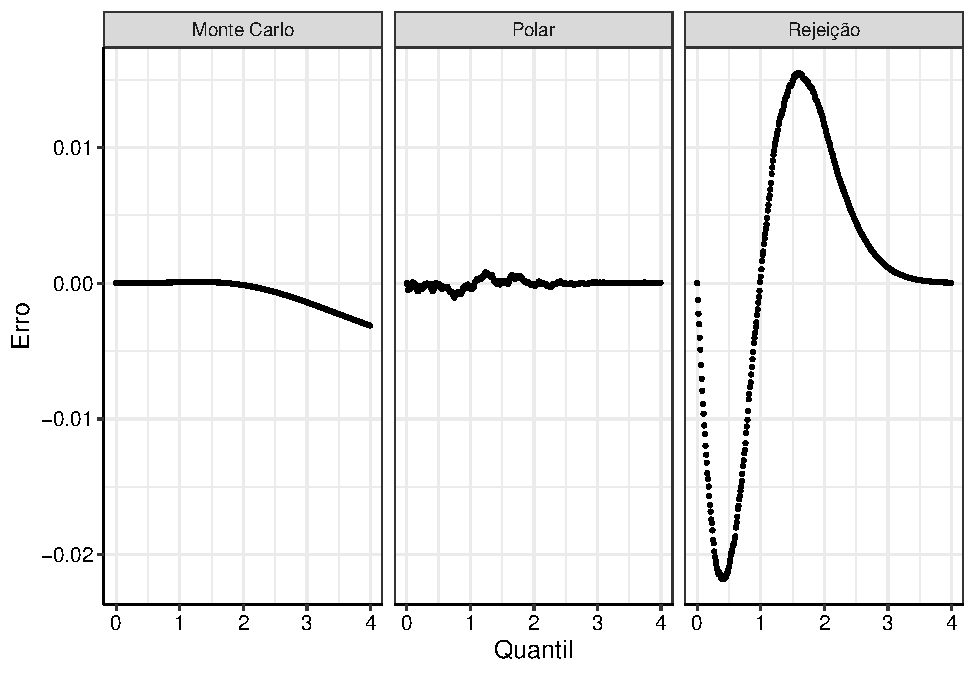
\includegraphics{relatorio_tp2_files/figure-latex/erros-estimacao-1.pdf}

\hypertarget{anexo-a---cuxf3digo-comentado}{%
\section*{Anexo A - código
comentado}\label{anexo-a---cuxf3digo-comentado}}
\addcontentsline{toc}{section}{Anexo A - código comentado}

\begin{Shaded}
\begin{Highlighting}[]
\CommentTok{\# VA UNIFORME}
\NormalTok{uniforme }\OtherTok{\textless{}{-}} \ControlFlowTok{function}\NormalTok{(n)\{}
  
\NormalTok{  x }\OtherTok{\textless{}{-}} \FunctionTok{c}\NormalTok{()}
  
\NormalTok{  a }\OtherTok{\textless{}{-}} \DecValTok{16807}
\NormalTok{  m }\OtherTok{\textless{}{-}} \DecValTok{2}\SpecialCharTok{\^{}}\DecValTok{31} \SpecialCharTok{{-}}\DecValTok{1}
  
  \CommentTok{\# se tem o arquivo com seed, pega o seed k do arquivo}
  \CommentTok{\# Se nao tiver arquivo, gera o arquivo e escreve o seed}
  \CommentTok{\# seed começa com o relogio}
  \CommentTok{\# Os que extrapolarem inserir no arquivo}
  
  \ControlFlowTok{if}\NormalTok{ (}\FunctionTok{file.exists}\NormalTok{(}\StringTok{"../trabalho pratico 2/seeds.Rdata"}\NormalTok{))\{}
\NormalTok{    y }\OtherTok{\textless{}{-}} \FunctionTok{readRDS}\NormalTok{(}\StringTok{"../trabalho pratico 2/seeds.Rdata"}\NormalTok{)}
\NormalTok{  \} }\ControlFlowTok{else}\NormalTok{ \{}
\NormalTok{    y }\OtherTok{\textless{}{-}} \FunctionTok{as.numeric}\NormalTok{(}\FunctionTok{Sys.time}\NormalTok{())}
\NormalTok{  \}}
  
  \ControlFlowTok{for}\NormalTok{ (i }\ControlFlowTok{in} \DecValTok{1}\SpecialCharTok{:}\NormalTok{n)\{}
\NormalTok{    y }\OtherTok{\textless{}{-}}\NormalTok{ (a}\SpecialCharTok{*}\NormalTok{y)}\SpecialCharTok{\%\%}\NormalTok{m}
\NormalTok{    x[i] }\OtherTok{\textless{}{-}}\NormalTok{ y}\SpecialCharTok{/}\NormalTok{m}
\NormalTok{  \}}
  
  \CommentTok{\#guardar o ultimo y num arquivo}
  \FunctionTok{saveRDS}\NormalTok{(y, }\StringTok{"../trabalho pratico 2/seeds.Rdata"}\NormalTok{)}
  
  \FunctionTok{return}\NormalTok{(x)}
\NormalTok{\}}

\CommentTok{\# VA POISSON}
\NormalTok{poisson }\OtherTok{\textless{}{-}} \ControlFlowTok{function}\NormalTok{(lambda)\{}
  
  \ControlFlowTok{if}\NormalTok{(}\SpecialCharTok{!}\FunctionTok{is.integer}\NormalTok{(lambda))\{}
    \FunctionTok{message}\NormalTok{(}\StringTok{"Usando a parte inteira do lambda fornecido."}\NormalTok{)}
\NormalTok{    lambda }\OtherTok{\textless{}{-}} \FunctionTok{as.integer}\NormalTok{(lambda)}
\NormalTok{  \}}
  
\NormalTok{  p }\OtherTok{\textless{}{-}} \FunctionTok{exp}\NormalTok{(}\SpecialCharTok{{-}}\NormalTok{lambda)}
\NormalTok{  U }\OtherTok{\textless{}{-}} \FunctionTok{uniforme}\NormalTok{(}\DecValTok{1}\NormalTok{)}
\NormalTok{  f }\OtherTok{\textless{}{-}}\NormalTok{ p}
  
\NormalTok{  i }\OtherTok{\textless{}{-}} \DecValTok{0}
  
  \CommentTok{\# testa se o número está na média}
    \ControlFlowTok{while}\NormalTok{ (U }\SpecialCharTok{\textgreater{}=}\NormalTok{ f)\{}
\NormalTok{      p }\OtherTok{\textless{}{-}}\NormalTok{ (p}\SpecialCharTok{*}\NormalTok{lambda)}\SpecialCharTok{/}\NormalTok{(i}\SpecialCharTok{+}\DecValTok{1}\NormalTok{)}
\NormalTok{      f }\OtherTok{\textless{}{-}}\NormalTok{ f}\SpecialCharTok{+}\NormalTok{p}
\NormalTok{      i }\OtherTok{\textless{}{-}}\NormalTok{ i}\SpecialCharTok{+}\DecValTok{1}
\NormalTok{    \}}
    \FunctionTok{return}\NormalTok{(i)}
\NormalTok{\}}

\CommentTok{\# VA EXPONENCIAL}
\NormalTok{geraexp }\OtherTok{\textless{}{-}} \ControlFlowTok{function}\NormalTok{(n, lambda)\{}
\NormalTok{  u }\OtherTok{\textless{}{-}} \FunctionTok{uniforme}\NormalTok{(n)}
  
\NormalTok{  saida }\OtherTok{\textless{}{-}} \SpecialCharTok{{-}}\FunctionTok{log}\NormalTok{(u)}\SpecialCharTok{/}\NormalTok{lambda}
  
  \FunctionTok{return}\NormalTok{(saida)}
\NormalTok{\}}

\CommentTok{\# VA NORMAL}
\NormalTok{geranormal }\OtherTok{\textless{}{-}} \ControlFlowTok{function}\NormalTok{(metodo)\{}
  \ControlFlowTok{if}\NormalTok{ (metodo }\SpecialCharTok{==} \StringTok{"rejeicao"}\NormalTok{)\{}
\NormalTok{    y }\OtherTok{\textless{}{-}} \FunctionTok{geraexp}\NormalTok{(}\AttributeTok{n =} \DecValTok{1}\NormalTok{, }\AttributeTok{lambda =} \DecValTok{1}\NormalTok{)}
\NormalTok{    u }\OtherTok{\textless{}{-}} \FunctionTok{uniforme}\NormalTok{(}\DecValTok{1}\NormalTok{)}
    \ControlFlowTok{while}\NormalTok{(u }\SpecialCharTok{\textgreater{}} \FunctionTok{exp}\NormalTok{(}\SpecialCharTok{{-}}\NormalTok{(y}\DecValTok{{-}1}\NormalTok{)}\SpecialCharTok{\^{}}\DecValTok{2}\NormalTok{)}\SpecialCharTok{/}\DecValTok{2}\NormalTok{)\{}
\NormalTok{      u }\OtherTok{\textless{}{-}} \FunctionTok{uniforme}\NormalTok{(}\DecValTok{1}\NormalTok{)}
\NormalTok{      y }\OtherTok{\textless{}{-}} \FunctionTok{geraexp}\NormalTok{(}\AttributeTok{n =} \DecValTok{1}\NormalTok{, }\AttributeTok{lambda =} \DecValTok{1}\NormalTok{)}
\NormalTok{    \}}
\NormalTok{    modZ }\OtherTok{\textless{}{-}} \FunctionTok{abs}\NormalTok{(y)}
    
    \ControlFlowTok{if}\NormalTok{(}\FunctionTok{uniforme}\NormalTok{(}\DecValTok{1}\NormalTok{) }\SpecialCharTok{\textless{}=} \FloatTok{0.5}\NormalTok{)\{}
\NormalTok{      Z }\OtherTok{\textless{}{-}}\NormalTok{ modZ}
\NormalTok{    \} }\ControlFlowTok{else}\NormalTok{ \{}
\NormalTok{      Z }\OtherTok{\textless{}{-}} \SpecialCharTok{{-}}\NormalTok{modZ}
\NormalTok{    \}}
    \FunctionTok{return}\NormalTok{(Z)}
\NormalTok{  \}}
  
  \ControlFlowTok{if}\NormalTok{(metodo }\SpecialCharTok{==} \StringTok{"polar"}\NormalTok{)\{}
\NormalTok{    v1 }\OtherTok{\textless{}{-}}\NormalTok{ (}\DecValTok{2}\SpecialCharTok{*}\FunctionTok{uniforme}\NormalTok{(}\DecValTok{1}\NormalTok{)}\SpecialCharTok{{-}}\DecValTok{1}\NormalTok{)}
\NormalTok{    v2 }\OtherTok{\textless{}{-}}\NormalTok{ (}\DecValTok{2}\SpecialCharTok{*}\FunctionTok{uniforme}\NormalTok{(}\DecValTok{1}\NormalTok{)}\SpecialCharTok{{-}}\DecValTok{1}\NormalTok{)}
\NormalTok{    u }\OtherTok{\textless{}{-}}\NormalTok{ v1}\SpecialCharTok{\^{}}\DecValTok{2} \SpecialCharTok{+}\NormalTok{ v2}\SpecialCharTok{\^{}}\DecValTok{2}
    \ControlFlowTok{while}\NormalTok{ (u }\SpecialCharTok{\textgreater{}} \DecValTok{1}\NormalTok{)\{}
\NormalTok{      v1 }\OtherTok{\textless{}{-}}\NormalTok{ (}\DecValTok{2}\SpecialCharTok{*}\FunctionTok{uniforme}\NormalTok{(}\DecValTok{1}\NormalTok{)}\SpecialCharTok{{-}}\DecValTok{1}\NormalTok{)}
\NormalTok{      v2 }\OtherTok{\textless{}{-}}\NormalTok{ (}\DecValTok{2}\SpecialCharTok{*}\FunctionTok{uniforme}\NormalTok{(}\DecValTok{1}\NormalTok{)}\SpecialCharTok{{-}}\DecValTok{1}\NormalTok{)}
\NormalTok{      u }\OtherTok{\textless{}{-}}\NormalTok{ v1}\SpecialCharTok{\^{}}\DecValTok{2} \SpecialCharTok{+}\NormalTok{ v2}\SpecialCharTok{\^{}}\DecValTok{2}
\NormalTok{    \}}
\NormalTok{    x }\OtherTok{\textless{}{-}} \FunctionTok{sqrt}\NormalTok{(}\SpecialCharTok{{-}}\DecValTok{2}\SpecialCharTok{*}\FunctionTok{log}\NormalTok{(u)}\SpecialCharTok{/}\NormalTok{u)}\SpecialCharTok{*}\NormalTok{v1}
\NormalTok{    y }\OtherTok{\textless{}{-}} \FunctionTok{sqrt}\NormalTok{(}\SpecialCharTok{{-}}\DecValTok{2}\SpecialCharTok{*}\FunctionTok{log}\NormalTok{(u)}\SpecialCharTok{/}\NormalTok{u)}\SpecialCharTok{*}\NormalTok{v2}
    \FunctionTok{return}\NormalTok{(}\FunctionTok{list}\NormalTok{(}\AttributeTok{x =}\NormalTok{ x, }\AttributeTok{y =}\NormalTok{ y))}
\NormalTok{  \}}
\NormalTok{\}}

\CommentTok{\# GERACAO DE AMOSTRAS}
\ControlFlowTok{if}\NormalTok{(}\SpecialCharTok{!}\FunctionTok{file.exists}\NormalTok{(}\StringTok{"../trabalho pratico 2/amostra\_uniforme.Rdata"}\NormalTok{))\{}
  \CommentTok{\# uniforme}
\NormalTok{  am\_uni }\OtherTok{\textless{}{-}} \FunctionTok{data.frame}\NormalTok{(}\AttributeTok{amostra =} \FunctionTok{uniforme}\NormalTok{(}\DecValTok{200000}\NormalTok{))}
  
  \CommentTok{\# poisson lambda = 1}
\NormalTok{  am\_poisson }\OtherTok{\textless{}{-}} \FunctionTok{c}\NormalTok{()}
  \ControlFlowTok{for}\NormalTok{ (i }\ControlFlowTok{in} \DecValTok{1}\SpecialCharTok{:}\DecValTok{200000}\NormalTok{)\{}
\NormalTok{    am\_poisson[i] }\OtherTok{\textless{}{-}} \FunctionTok{poisson}\NormalTok{(1L)}
\NormalTok{  \}}
\NormalTok{  am\_poisson }\OtherTok{\textless{}{-}} \FunctionTok{data.frame}\NormalTok{(}\AttributeTok{amostra =}\NormalTok{ am\_poisson)}
  
  \CommentTok{\# exponencial lambda 1}
\NormalTok{  am\_exp }\OtherTok{\textless{}{-}} \FunctionTok{data.frame}\NormalTok{(}\AttributeTok{amostra =} \FunctionTok{geraexp}\NormalTok{(}\DecValTok{200000}\NormalTok{, }\DecValTok{1}\NormalTok{))}
  
  \CommentTok{\# normal rejeição}
\NormalTok{  am\_normrej }\OtherTok{\textless{}{-}} \FunctionTok{c}\NormalTok{()}
  \ControlFlowTok{for}\NormalTok{ (i }\ControlFlowTok{in} \DecValTok{1}\SpecialCharTok{:}\DecValTok{200000}\NormalTok{)\{}
\NormalTok{    am\_normrej[i] }\OtherTok{\textless{}{-}} \FunctionTok{geranormal}\NormalTok{(}\StringTok{"rejeicao"}\NormalTok{)}
\NormalTok{  \}}
\NormalTok{  am\_normrej }\OtherTok{\textless{}{-}} \FunctionTok{data.frame}\NormalTok{(}\AttributeTok{amostra =}\NormalTok{ am\_normrej)}
  
  \CommentTok{\# normal polar}
\NormalTok{  x }\OtherTok{\textless{}{-}} \FunctionTok{c}\NormalTok{()}
\NormalTok{  y }\OtherTok{\textless{}{-}} \FunctionTok{c}\NormalTok{()}
  \ControlFlowTok{for}\NormalTok{ (i }\ControlFlowTok{in} \DecValTok{1}\SpecialCharTok{:}\DecValTok{200000}\NormalTok{)\{}
\NormalTok{    x[i] }\OtherTok{\textless{}{-}} \FunctionTok{geranormal}\NormalTok{(}\StringTok{"polar"}\NormalTok{)}\SpecialCharTok{$}\NormalTok{x}
\NormalTok{    y[i] }\OtherTok{\textless{}{-}} \FunctionTok{geranormal}\NormalTok{(}\StringTok{"polar"}\NormalTok{)}\SpecialCharTok{$}\NormalTok{y}
\NormalTok{  \}}
  
\NormalTok{  am\_normpolar }\OtherTok{\textless{}{-}} \FunctionTok{data.frame}\NormalTok{(}\AttributeTok{x =}\NormalTok{ x, }\AttributeTok{y =}\NormalTok{ y)}
  \FunctionTok{rm}\NormalTok{(x,y,i)}
  
  \FunctionTok{saveRDS}\NormalTok{(am\_uni, }\StringTok{"../trabalho pratico 2/amostra\_uniforme.Rdata"}\NormalTok{)}
  \FunctionTok{saveRDS}\NormalTok{(am\_poisson, }\StringTok{"../trabalho pratico 2/amostra\_poisson.Rdata"}\NormalTok{)}
  \FunctionTok{saveRDS}\NormalTok{(am\_exp, }\StringTok{"../trabalho pratico 2/amostra\_exponencial.Rdata"}\NormalTok{)}
  \FunctionTok{saveRDS}\NormalTok{(am\_normrej, }\StringTok{"../trabalho pratico 2/amostra\_normal\_rejeicao.Rdata"}\NormalTok{)}
  \FunctionTok{saveRDS}\NormalTok{(am\_normpolar, }\StringTok{"../trabalho pratico 2/amostra\_normal\_polar.Rdata"}\NormalTok{)}
\NormalTok{\} }\ControlFlowTok{else}\NormalTok{ \{}
\NormalTok{  am\_uni }\OtherTok{\textless{}{-}} \FunctionTok{readRDS}\NormalTok{(}\StringTok{"../trabalho pratico 2/amostra\_uniforme.Rdata"}\NormalTok{)}
\NormalTok{  am\_poisson }\OtherTok{\textless{}{-}} \FunctionTok{readRDS}\NormalTok{(}\StringTok{"../trabalho pratico 2/amostra\_poisson.Rdata"}\NormalTok{)}
\NormalTok{  am\_exp }\OtherTok{\textless{}{-}} \FunctionTok{readRDS}\NormalTok{(}\StringTok{"../trabalho pratico 2/amostra\_exponencial.Rdata"}\NormalTok{)}
\NormalTok{  am\_normrej }\OtherTok{\textless{}{-}} \FunctionTok{readRDS}\NormalTok{(}\StringTok{"../trabalho pratico 2/amostra\_normal\_rejeicao.Rdata"}\NormalTok{)}
\NormalTok{  am\_normpolar }\OtherTok{\textless{}{-}} \FunctionTok{readRDS}\NormalTok{(}\StringTok{"../trabalho pratico 2/amostra\_normal\_polar.Rdata"}\NormalTok{)}
\NormalTok{\}}

\CommentTok{\# GRAFICO E TESTE UNIFORME}
\FunctionTok{ggplot}\NormalTok{(am\_uni, }\FunctionTok{aes}\NormalTok{(amostra))}\SpecialCharTok{+}
  \FunctionTok{geom\_histogram}\NormalTok{(}\FunctionTok{aes}\NormalTok{(}\AttributeTok{y =}\NormalTok{ ..density..),}\AttributeTok{color =} \StringTok{\textquotesingle{}white\textquotesingle{}}\NormalTok{)}\SpecialCharTok{+}
  \FunctionTok{stat\_function}\NormalTok{(}\AttributeTok{fun =}\NormalTok{ dunif, }\AttributeTok{color =} \StringTok{\textquotesingle{}red\textquotesingle{}}\NormalTok{, }\AttributeTok{args =} \FunctionTok{list}\NormalTok{(}\AttributeTok{min =} \DecValTok{0}\NormalTok{, }\AttributeTok{max =} \DecValTok{1}\NormalTok{), }\AttributeTok{size =} \FloatTok{0.7}\NormalTok{)}\SpecialCharTok{+}
  \FunctionTok{labs}\NormalTok{(}\AttributeTok{x =} \StringTok{"Amostra"}\NormalTok{, }\AttributeTok{y =} \StringTok{"Densidade"}\NormalTok{)}\SpecialCharTok{+}
  \FunctionTok{scale\_y\_continuous}\NormalTok{(}\AttributeTok{expand =} \FunctionTok{c}\NormalTok{(}\DecValTok{0}\NormalTok{,}\DecValTok{0}\NormalTok{))}\SpecialCharTok{+}
  \FunctionTok{theme\_bw}\NormalTok{() }\SpecialCharTok{+}
  \FunctionTok{theme}\NormalTok{(}\AttributeTok{axis.title.y=}\FunctionTok{element\_text}\NormalTok{(}\AttributeTok{colour=}\StringTok{"black"}\NormalTok{, }\AttributeTok{size=}\DecValTok{12}\NormalTok{),}
        \AttributeTok{axis.title.x =} \FunctionTok{element\_text}\NormalTok{(}\AttributeTok{colour=}\StringTok{"black"}\NormalTok{, }\AttributeTok{size=}\DecValTok{12}\NormalTok{),}
        \AttributeTok{axis.text =} \FunctionTok{element\_text}\NormalTok{(}\AttributeTok{colour =} \StringTok{"black"}\NormalTok{, }\AttributeTok{size=}\FloatTok{9.5}\NormalTok{),}
        \AttributeTok{panel.border =} \FunctionTok{element\_blank}\NormalTok{(),}
        \AttributeTok{axis.line =} \FunctionTok{element\_line}\NormalTok{(}\AttributeTok{colour =} \StringTok{"black"}\NormalTok{),}
        \AttributeTok{panel.grid =} \FunctionTok{element\_blank}\NormalTok{()) }

\NormalTok{q1 }\OtherTok{\textless{}{-}} \FunctionTok{sum}\NormalTok{(am\_uni}\SpecialCharTok{$}\NormalTok{amostra }\SpecialCharTok{\textless{}}\NormalTok{ .}\DecValTok{25}\NormalTok{)}
\NormalTok{q2 }\OtherTok{\textless{}{-}} \FunctionTok{sum}\NormalTok{(am\_uni}\SpecialCharTok{$}\NormalTok{amostra  }\SpecialCharTok{\textgreater{}=}\NormalTok{ .}\DecValTok{25} \SpecialCharTok{\&}\NormalTok{ am\_uni}\SpecialCharTok{$}\NormalTok{amostra }\SpecialCharTok{\textless{}}\NormalTok{ .}\DecValTok{5}\NormalTok{)}
\NormalTok{q3 }\OtherTok{\textless{}{-}} \FunctionTok{sum}\NormalTok{(am\_uni}\SpecialCharTok{$}\NormalTok{amostra  }\SpecialCharTok{\textgreater{}=}\NormalTok{ .}\DecValTok{5} \SpecialCharTok{\&}\NormalTok{ am\_uni}\SpecialCharTok{$}\NormalTok{amostra }\SpecialCharTok{\textless{}}\NormalTok{ .}\DecValTok{75}\NormalTok{)}
\NormalTok{q4 }\OtherTok{\textless{}{-}} \FunctionTok{sum}\NormalTok{(am\_uni}\SpecialCharTok{$}\NormalTok{amostra  }\SpecialCharTok{\textgreater{}=}\NormalTok{ .}\DecValTok{75} \SpecialCharTok{\&}\NormalTok{ am\_uni}\SpecialCharTok{$}\NormalTok{amostra }\SpecialCharTok{\textless{}=} \DecValTok{1}\NormalTok{)}

\NormalTok{quartis }\OtherTok{\textless{}{-}} \FunctionTok{c}\NormalTok{(q1,q2, q3, q4)}\SpecialCharTok{/}\DecValTok{2000}

\NormalTok{pvalor }\OtherTok{\textless{}{-}} \FunctionTok{chisq.test}\NormalTok{(quartis, }\AttributeTok{p =} \FunctionTok{c}\NormalTok{(.}\DecValTok{25}\NormalTok{, .}\DecValTok{25}\NormalTok{, .}\DecValTok{25}\NormalTok{, .}\DecValTok{25}\NormalTok{))}\SpecialCharTok{$}\NormalTok{p.value}

\CommentTok{\# GRAFICO E TESTE POISSON}
\NormalTok{x.values }\OtherTok{\textless{}{-}} \FunctionTok{seq}\NormalTok{(}\DecValTok{0}\NormalTok{, }\DecValTok{10}\NormalTok{, }\DecValTok{1}\NormalTok{)}
\NormalTok{y2 }\OtherTok{\textless{}{-}} \FunctionTok{dpois}\NormalTok{(x.values, }\DecValTok{1}\NormalTok{)}
\NormalTok{df2 }\OtherTok{\textless{}{-}} \FunctionTok{data.frame}\NormalTok{(x.values, y2)}

\FunctionTok{ggplot}\NormalTok{(df2, }\FunctionTok{aes}\NormalTok{(}\AttributeTok{x=}\NormalTok{x.values, }\AttributeTok{y=}\NormalTok{y2))}\SpecialCharTok{+}
  \FunctionTok{geom\_histogram}\NormalTok{(}\AttributeTok{data =}\NormalTok{ am\_poisson, }\FunctionTok{aes}\NormalTok{(}\AttributeTok{x =}\NormalTok{ amostra, }\AttributeTok{y =}\NormalTok{ ..density..),}\AttributeTok{color =} \StringTok{\textquotesingle{}white\textquotesingle{}}\NormalTok{, }\AttributeTok{bins =} \DecValTok{10}\NormalTok{)}\SpecialCharTok{+}
  \FunctionTok{geom\_point}\NormalTok{(}\AttributeTok{stat=}\StringTok{"identity"}\NormalTok{, }\AttributeTok{width =} \FloatTok{0.5}\NormalTok{, }\AttributeTok{color =} \StringTok{"red"}\NormalTok{)}\SpecialCharTok{+}
  \FunctionTok{geom\_line}\NormalTok{(}\AttributeTok{color =} \StringTok{"red"}\NormalTok{)}\SpecialCharTok{+}
  \FunctionTok{labs}\NormalTok{(}\AttributeTok{x =} \StringTok{"Amostra"}\NormalTok{, }\AttributeTok{y =} \StringTok{"Densidade"}\NormalTok{)}\SpecialCharTok{+}
  \FunctionTok{scale\_y\_continuous}\NormalTok{(}\AttributeTok{expand =} \FunctionTok{c}\NormalTok{(}\DecValTok{0}\NormalTok{,}\DecValTok{0}\NormalTok{), }\AttributeTok{limits =} \FunctionTok{c}\NormalTok{(}\DecValTok{0}\NormalTok{, .}\DecValTok{4}\NormalTok{))}\SpecialCharTok{+}
  \FunctionTok{scale\_x\_continuous}\NormalTok{(}\AttributeTok{breaks =} \FunctionTok{c}\NormalTok{(}\DecValTok{0}\SpecialCharTok{:}\DecValTok{10}\NormalTok{), }\AttributeTok{expand =} \FunctionTok{c}\NormalTok{(}\DecValTok{0}\NormalTok{, }\FloatTok{0.2}\NormalTok{))}\SpecialCharTok{+}
  \FunctionTok{theme\_bw}\NormalTok{() }\SpecialCharTok{+}
  \FunctionTok{theme}\NormalTok{(}\AttributeTok{axis.title.y=}\FunctionTok{element\_text}\NormalTok{(}\AttributeTok{colour=}\StringTok{"black"}\NormalTok{, }\AttributeTok{size=}\DecValTok{12}\NormalTok{),}
        \AttributeTok{axis.title.x =} \FunctionTok{element\_text}\NormalTok{(}\AttributeTok{colour=}\StringTok{"black"}\NormalTok{, }\AttributeTok{size=}\DecValTok{12}\NormalTok{),}
        \AttributeTok{axis.text =} \FunctionTok{element\_text}\NormalTok{(}\AttributeTok{colour =} \StringTok{"black"}\NormalTok{, }\AttributeTok{size=}\FloatTok{9.5}\NormalTok{),}
        \AttributeTok{panel.border =} \FunctionTok{element\_blank}\NormalTok{(),}
        \AttributeTok{axis.line =} \FunctionTok{element\_line}\NormalTok{(}\AttributeTok{colour =} \StringTok{"black"}\NormalTok{),}
        \AttributeTok{panel.grid =} \FunctionTok{element\_blank}\NormalTok{()) }

\NormalTok{q1 }\OtherTok{\textless{}{-}} \FunctionTok{sum}\NormalTok{(am\_poisson}\SpecialCharTok{$}\NormalTok{amostra }\SpecialCharTok{\textless{}=} \FunctionTok{qpois}\NormalTok{(.}\DecValTok{25}\NormalTok{, }\AttributeTok{lambda =} \DecValTok{1}\NormalTok{))}
\NormalTok{q2 }\OtherTok{\textless{}{-}} \FunctionTok{sum}\NormalTok{(am\_poisson}\SpecialCharTok{$}\NormalTok{amostra  }\SpecialCharTok{\textgreater{}} \FunctionTok{qpois}\NormalTok{(.}\DecValTok{25}\NormalTok{, }\AttributeTok{lambda =} \DecValTok{1}\NormalTok{) }\SpecialCharTok{\&}\NormalTok{ am\_poisson}\SpecialCharTok{$}\NormalTok{amostra }\SpecialCharTok{\textless{}=} \FunctionTok{qpois}\NormalTok{(.}\DecValTok{5}\NormalTok{, }\AttributeTok{lambda =} \DecValTok{1}\NormalTok{))}
\NormalTok{q3 }\OtherTok{\textless{}{-}} \FunctionTok{sum}\NormalTok{(am\_poisson}\SpecialCharTok{$}\NormalTok{amostra  }\SpecialCharTok{\textgreater{}} \FunctionTok{qpois}\NormalTok{(.}\DecValTok{5}\NormalTok{, }\AttributeTok{lambda =} \DecValTok{1}\NormalTok{) }\SpecialCharTok{\&}\NormalTok{ am\_poisson}\SpecialCharTok{$}\NormalTok{amostra }\SpecialCharTok{\textless{}=} \FunctionTok{qpois}\NormalTok{(.}\DecValTok{75}\NormalTok{, }\AttributeTok{lambda =} \DecValTok{1}\NormalTok{))}
\NormalTok{q4 }\OtherTok{\textless{}{-}} \FunctionTok{sum}\NormalTok{(am\_poisson}\SpecialCharTok{$}\NormalTok{amostra  }\SpecialCharTok{\textgreater{}} \FunctionTok{qpois}\NormalTok{(.}\DecValTok{75}\NormalTok{, }\AttributeTok{lambda =} \DecValTok{1}\NormalTok{))}

\NormalTok{quartis }\OtherTok{\textless{}{-}} \FunctionTok{c}\NormalTok{(q1,q2, q3, q4)}\SpecialCharTok{/}\DecValTok{2000}

\NormalTok{p }\OtherTok{\textless{}{-}} \FunctionTok{c}\NormalTok{(}\FunctionTok{dpois}\NormalTok{(}\DecValTok{0}\NormalTok{, }\AttributeTok{lambda =} \DecValTok{1}\NormalTok{),}\FunctionTok{dpois}\NormalTok{(}\DecValTok{1}\NormalTok{, }\AttributeTok{lambda =} \DecValTok{1}\NormalTok{), }\FunctionTok{dpois}\NormalTok{(}\DecValTok{2}\NormalTok{, }\AttributeTok{lambda =} \DecValTok{1}\NormalTok{))}
\NormalTok{p[}\DecValTok{4}\NormalTok{] }\OtherTok{\textless{}{-}} \DecValTok{1}\SpecialCharTok{{-}}\FunctionTok{sum}\NormalTok{(p)}

\NormalTok{pvalor }\OtherTok{\textless{}{-}} \FunctionTok{chisq.test}\NormalTok{(quartis, }\AttributeTok{p =}\NormalTok{ p)}\SpecialCharTok{$}\NormalTok{p.value}

\CommentTok{\# GRAFICO E TESTE EXPONENCIAL}

\FunctionTok{ggplot}\NormalTok{(am\_exp, }\FunctionTok{aes}\NormalTok{(amostra))}\SpecialCharTok{+}
  \FunctionTok{geom\_histogram}\NormalTok{(}\FunctionTok{aes}\NormalTok{(}\AttributeTok{y =}\NormalTok{ ..density..),}\AttributeTok{color =} \StringTok{\textquotesingle{}white\textquotesingle{}}\NormalTok{)}\SpecialCharTok{+}
  \FunctionTok{stat\_function}\NormalTok{(}\AttributeTok{fun =}\NormalTok{ dexp, }\AttributeTok{color =} \StringTok{\textquotesingle{}red\textquotesingle{}}\NormalTok{, }\AttributeTok{args =} \FunctionTok{list}\NormalTok{(}\DecValTok{1}\NormalTok{))}\SpecialCharTok{+}
  \FunctionTok{labs}\NormalTok{(}\AttributeTok{x =} \StringTok{"Amostra"}\NormalTok{, }\AttributeTok{y =} \StringTok{"Densidade"}\NormalTok{)}\SpecialCharTok{+}
  \FunctionTok{scale\_y\_continuous}\NormalTok{(}\AttributeTok{expand =} \FunctionTok{c}\NormalTok{(}\DecValTok{0}\NormalTok{,}\DecValTok{0}\NormalTok{))}\SpecialCharTok{+}
  \FunctionTok{theme\_bw}\NormalTok{() }\SpecialCharTok{+}
  \FunctionTok{theme}\NormalTok{(}\AttributeTok{axis.title.y=}\FunctionTok{element\_text}\NormalTok{(}\AttributeTok{colour=}\StringTok{"black"}\NormalTok{, }\AttributeTok{size=}\DecValTok{12}\NormalTok{),}
        \AttributeTok{axis.title.x =} \FunctionTok{element\_text}\NormalTok{(}\AttributeTok{colour=}\StringTok{"black"}\NormalTok{, }\AttributeTok{size=}\DecValTok{12}\NormalTok{),}
        \AttributeTok{axis.text =} \FunctionTok{element\_text}\NormalTok{(}\AttributeTok{colour =} \StringTok{"black"}\NormalTok{, }\AttributeTok{size=}\FloatTok{9.5}\NormalTok{),}
        \AttributeTok{panel.border =} \FunctionTok{element\_blank}\NormalTok{(),}
        \AttributeTok{axis.line =} \FunctionTok{element\_line}\NormalTok{(}\AttributeTok{colour =} \StringTok{"black"}\NormalTok{),}
        \AttributeTok{panel.grid =} \FunctionTok{element\_blank}\NormalTok{()) }

\NormalTok{q1 }\OtherTok{\textless{}{-}} \FunctionTok{sum}\NormalTok{(am\_exp}\SpecialCharTok{$}\NormalTok{amostra }\SpecialCharTok{\textless{}=} \FunctionTok{qexp}\NormalTok{(.}\DecValTok{25}\NormalTok{, }\AttributeTok{rate =} \DecValTok{1}\NormalTok{))}
\NormalTok{q2 }\OtherTok{\textless{}{-}} \FunctionTok{sum}\NormalTok{(am\_exp}\SpecialCharTok{$}\NormalTok{amostra  }\SpecialCharTok{\textgreater{}} \FunctionTok{qexp}\NormalTok{(.}\DecValTok{25}\NormalTok{, }\AttributeTok{rate =} \DecValTok{1}\NormalTok{) }\SpecialCharTok{\&}\NormalTok{ am\_exp}\SpecialCharTok{$}\NormalTok{amostra }\SpecialCharTok{\textless{}=} \FunctionTok{qexp}\NormalTok{(.}\DecValTok{5}\NormalTok{, }\AttributeTok{rate =} \DecValTok{1}\NormalTok{))}
\NormalTok{q3 }\OtherTok{\textless{}{-}} \FunctionTok{sum}\NormalTok{(am\_exp}\SpecialCharTok{$}\NormalTok{amostra  }\SpecialCharTok{\textgreater{}} \FunctionTok{qexp}\NormalTok{(.}\DecValTok{5}\NormalTok{, }\AttributeTok{rate =} \DecValTok{1}\NormalTok{) }\SpecialCharTok{\&}\NormalTok{ am\_exp}\SpecialCharTok{$}\NormalTok{amostra }\SpecialCharTok{\textless{}=} \FunctionTok{qexp}\NormalTok{(.}\DecValTok{75}\NormalTok{, }\AttributeTok{rate =} \DecValTok{1}\NormalTok{))}
\NormalTok{q4 }\OtherTok{\textless{}{-}} \FunctionTok{sum}\NormalTok{(am\_exp}\SpecialCharTok{$}\NormalTok{amostra  }\SpecialCharTok{\textgreater{}} \FunctionTok{qexp}\NormalTok{(.}\DecValTok{75}\NormalTok{, }\AttributeTok{rate =} \DecValTok{1}\NormalTok{))}

\NormalTok{quartis }\OtherTok{\textless{}{-}} \FunctionTok{c}\NormalTok{(q1,q2, q3, q4)}\SpecialCharTok{/}\DecValTok{2000}

\NormalTok{pvalor }\OtherTok{\textless{}{-}} \FunctionTok{chisq.test}\NormalTok{(quartis, }\AttributeTok{p =} \FunctionTok{c}\NormalTok{(.}\DecValTok{25}\NormalTok{, .}\DecValTok{25}\NormalTok{, .}\DecValTok{25}\NormalTok{, .}\DecValTok{25}\NormalTok{))}\SpecialCharTok{$}\NormalTok{p.value}

\CommentTok{\# GRAFICO E TESTE NORMAL}

\FunctionTok{ggplot}\NormalTok{(am\_normrej, }\FunctionTok{aes}\NormalTok{(amostra))}\SpecialCharTok{+}
  \FunctionTok{geom\_histogram}\NormalTok{(}\FunctionTok{aes}\NormalTok{(}\AttributeTok{y =}\NormalTok{ ..density..),}\AttributeTok{color =} \StringTok{\textquotesingle{}white\textquotesingle{}}\NormalTok{)}\SpecialCharTok{+}
  \FunctionTok{stat\_function}\NormalTok{(}\AttributeTok{fun =}\NormalTok{ dnorm, }\AttributeTok{color =} \StringTok{\textquotesingle{}red\textquotesingle{}}\NormalTok{, }\AttributeTok{args =} \FunctionTok{list}\NormalTok{(}\AttributeTok{mean =} \DecValTok{0}\NormalTok{, }\AttributeTok{sd =} \DecValTok{1}\NormalTok{))}\SpecialCharTok{+}
  \FunctionTok{labs}\NormalTok{(}\AttributeTok{x =} \StringTok{"Amostra"}\NormalTok{, }\AttributeTok{y =} \StringTok{"Densidade"}\NormalTok{)}\SpecialCharTok{+}
  \FunctionTok{scale\_y\_continuous}\NormalTok{(}\AttributeTok{expand =} \FunctionTok{c}\NormalTok{(}\DecValTok{0}\NormalTok{,}\DecValTok{0}\NormalTok{), }\AttributeTok{limits =} \FunctionTok{c}\NormalTok{(}\DecValTok{0}\NormalTok{, .}\DecValTok{42}\NormalTok{))}\SpecialCharTok{+}
  \FunctionTok{theme\_bw}\NormalTok{() }\SpecialCharTok{+}
  \FunctionTok{theme}\NormalTok{(}\AttributeTok{axis.title.y=}\FunctionTok{element\_text}\NormalTok{(}\AttributeTok{colour=}\StringTok{"black"}\NormalTok{, }\AttributeTok{size=}\DecValTok{12}\NormalTok{),}
        \AttributeTok{axis.title.x =} \FunctionTok{element\_text}\NormalTok{(}\AttributeTok{colour=}\StringTok{"black"}\NormalTok{, }\AttributeTok{size=}\DecValTok{12}\NormalTok{),}
        \AttributeTok{axis.text =} \FunctionTok{element\_text}\NormalTok{(}\AttributeTok{colour =} \StringTok{"black"}\NormalTok{, }\AttributeTok{size=}\FloatTok{9.5}\NormalTok{),}
        \AttributeTok{panel.border =} \FunctionTok{element\_blank}\NormalTok{(),}
        \AttributeTok{axis.line =} \FunctionTok{element\_line}\NormalTok{(}\AttributeTok{colour =} \StringTok{"black"}\NormalTok{),}
        \AttributeTok{panel.grid =} \FunctionTok{element\_blank}\NormalTok{())}
\NormalTok{q1 }\OtherTok{\textless{}{-}} \FunctionTok{sum}\NormalTok{(am\_normrej}\SpecialCharTok{$}\NormalTok{amostra }\SpecialCharTok{\textless{}=} \FunctionTok{qnorm}\NormalTok{(.}\DecValTok{25}\NormalTok{))}
\NormalTok{q2 }\OtherTok{\textless{}{-}} \FunctionTok{sum}\NormalTok{(am\_normrej}\SpecialCharTok{$}\NormalTok{amostra  }\SpecialCharTok{\textgreater{}} \FunctionTok{qnorm}\NormalTok{(.}\DecValTok{25}\NormalTok{) }\SpecialCharTok{\&}\NormalTok{ am\_normrej}\SpecialCharTok{$}\NormalTok{amostra }\SpecialCharTok{\textless{}=} \FunctionTok{qnorm}\NormalTok{(.}\DecValTok{5}\NormalTok{))}
\NormalTok{q3 }\OtherTok{\textless{}{-}} \FunctionTok{sum}\NormalTok{(am\_normrej}\SpecialCharTok{$}\NormalTok{amostra  }\SpecialCharTok{\textgreater{}} \FunctionTok{qnorm}\NormalTok{(.}\DecValTok{5}\NormalTok{) }\SpecialCharTok{\&}\NormalTok{ am\_normrej}\SpecialCharTok{$}\NormalTok{amostra }\SpecialCharTok{\textless{}=} \FunctionTok{qnorm}\NormalTok{(.}\DecValTok{75}\NormalTok{))}
\NormalTok{q4 }\OtherTok{\textless{}{-}} \FunctionTok{sum}\NormalTok{(am\_normrej}\SpecialCharTok{$}\NormalTok{amostra  }\SpecialCharTok{\textgreater{}} \FunctionTok{qnorm}\NormalTok{(.}\DecValTok{75}\NormalTok{))}

\NormalTok{quartis }\OtherTok{\textless{}{-}} \FunctionTok{c}\NormalTok{(q1, q2, q3, q4)}\SpecialCharTok{/}\DecValTok{2000}

\NormalTok{pvalor }\OtherTok{\textless{}{-}} \FunctionTok{chisq.test}\NormalTok{(quartis, }\AttributeTok{p =} \FunctionTok{c}\NormalTok{(.}\DecValTok{25}\NormalTok{, .}\DecValTok{25}\NormalTok{, .}\DecValTok{25}\NormalTok{, .}\DecValTok{25}\NormalTok{))}\SpecialCharTok{$}\NormalTok{p.value}

\NormalTok{polar\_long }\OtherTok{\textless{}{-}}\NormalTok{ am\_normpolar }\SpecialCharTok{\%\textgreater{}\%}
  \FunctionTok{pivot\_longer}\NormalTok{(}\AttributeTok{cols =} \FunctionTok{everything}\NormalTok{(), }\AttributeTok{names\_to =} \StringTok{\textquotesingle{}eixo\textquotesingle{}}\NormalTok{, }\AttributeTok{values\_to =} \StringTok{\textquotesingle{}values\textquotesingle{}}\NormalTok{)}

\FunctionTok{ggplot}\NormalTok{(polar\_long, }\FunctionTok{aes}\NormalTok{(values))}\SpecialCharTok{+}
  \FunctionTok{geom\_histogram}\NormalTok{(}\FunctionTok{aes}\NormalTok{(}\AttributeTok{y =}\NormalTok{ ..density..),}\AttributeTok{color =} \StringTok{\textquotesingle{}white\textquotesingle{}}\NormalTok{)}\SpecialCharTok{+}
  \FunctionTok{stat\_function}\NormalTok{(}\AttributeTok{fun =}\NormalTok{ dnorm, }\AttributeTok{color =} \StringTok{\textquotesingle{}red\textquotesingle{}}\NormalTok{, }\AttributeTok{args =} \FunctionTok{list}\NormalTok{(}\AttributeTok{mean =} \DecValTok{0}\NormalTok{, }\AttributeTok{sd =} \DecValTok{1}\NormalTok{))}\SpecialCharTok{+}
  \FunctionTok{labs}\NormalTok{(}\AttributeTok{x =} \StringTok{"Amostra"}\NormalTok{, }\AttributeTok{y =} \StringTok{"Densidade"}\NormalTok{)}\SpecialCharTok{+}
  \FunctionTok{scale\_y\_continuous}\NormalTok{(}\AttributeTok{expand =} \FunctionTok{c}\NormalTok{(}\DecValTok{0}\NormalTok{,}\DecValTok{0}\NormalTok{), }\AttributeTok{limits =} \FunctionTok{c}\NormalTok{(}\DecValTok{0}\NormalTok{, .}\DecValTok{42}\NormalTok{))}\SpecialCharTok{+}
  \FunctionTok{theme\_bw}\NormalTok{() }\SpecialCharTok{+}
  \FunctionTok{theme}\NormalTok{(}\AttributeTok{axis.title.y=}\FunctionTok{element\_text}\NormalTok{(}\AttributeTok{colour=}\StringTok{"black"}\NormalTok{, }\AttributeTok{size=}\DecValTok{12}\NormalTok{),}
        \AttributeTok{axis.title.x =} \FunctionTok{element\_text}\NormalTok{(}\AttributeTok{colour=}\StringTok{"black"}\NormalTok{, }\AttributeTok{size=}\DecValTok{12}\NormalTok{),}
        \AttributeTok{axis.text =} \FunctionTok{element\_text}\NormalTok{(}\AttributeTok{colour =} \StringTok{"black"}\NormalTok{, }\AttributeTok{size=}\FloatTok{9.5}\NormalTok{),}
        \AttributeTok{panel.border =} \FunctionTok{element\_blank}\NormalTok{(),}
        \AttributeTok{axis.line =} \FunctionTok{element\_line}\NormalTok{(}\AttributeTok{colour =} \StringTok{"black"}\NormalTok{),}
        \AttributeTok{panel.grid =} \FunctionTok{element\_blank}\NormalTok{())}\SpecialCharTok{+}
  \FunctionTok{facet\_wrap}\NormalTok{(}\FunctionTok{vars}\NormalTok{(eixo),}\AttributeTok{ncol =} \DecValTok{2}\NormalTok{)}
\NormalTok{q1 }\OtherTok{\textless{}{-}} \FunctionTok{sum}\NormalTok{(am\_normpolar}\SpecialCharTok{$}\NormalTok{x }\SpecialCharTok{\textless{}=} \FunctionTok{qnorm}\NormalTok{(.}\DecValTok{25}\NormalTok{))}
\NormalTok{q2 }\OtherTok{\textless{}{-}} \FunctionTok{sum}\NormalTok{(am\_normpolar}\SpecialCharTok{$}\NormalTok{x  }\SpecialCharTok{\textgreater{}} \FunctionTok{qnorm}\NormalTok{(.}\DecValTok{25}\NormalTok{) }\SpecialCharTok{\&}\NormalTok{ am\_normpolar}\SpecialCharTok{$}\NormalTok{x }\SpecialCharTok{\textless{}=} \FunctionTok{qnorm}\NormalTok{(.}\DecValTok{5}\NormalTok{))}
\NormalTok{q3 }\OtherTok{\textless{}{-}} \FunctionTok{sum}\NormalTok{(am\_normpolar}\SpecialCharTok{$}\NormalTok{x  }\SpecialCharTok{\textgreater{}} \FunctionTok{qnorm}\NormalTok{(.}\DecValTok{5}\NormalTok{) }\SpecialCharTok{\&}\NormalTok{ am\_normpolar}\SpecialCharTok{$}\NormalTok{x }\SpecialCharTok{\textless{}=} \FunctionTok{qnorm}\NormalTok{(.}\DecValTok{75}\NormalTok{))}
\NormalTok{q4 }\OtherTok{\textless{}{-}} \FunctionTok{sum}\NormalTok{(am\_normpolar}\SpecialCharTok{$}\NormalTok{x  }\SpecialCharTok{\textgreater{}} \FunctionTok{qnorm}\NormalTok{(.}\DecValTok{75}\NormalTok{))}

\NormalTok{quartis }\OtherTok{\textless{}{-}} \FunctionTok{c}\NormalTok{(q1, q2, q3, q4)}\SpecialCharTok{/}\DecValTok{2000}

\NormalTok{pvalor }\OtherTok{\textless{}{-}} \FunctionTok{chisq.test}\NormalTok{(quartis, }\AttributeTok{p =} \FunctionTok{c}\NormalTok{(.}\DecValTok{25}\NormalTok{, .}\DecValTok{25}\NormalTok{, .}\DecValTok{25}\NormalTok{, .}\DecValTok{25}\NormalTok{))}\SpecialCharTok{$}\NormalTok{p.value}

\CommentTok{\# ESTIMACAO MONTECARLO}
\FunctionTok{set.seed}\NormalTok{(}\DecValTok{1234}\NormalTok{)}
\NormalTok{y }\OtherTok{\textless{}{-}} \FunctionTok{runif}\NormalTok{(}\DecValTok{10000}\NormalTok{)}

\NormalTok{acumulada\_normal }\OtherTok{\textless{}{-}} \ControlFlowTok{function}\NormalTok{(b, }\AttributeTok{n=}\DecValTok{10000}\NormalTok{)\{}
\NormalTok{  h }\OtherTok{\textless{}{-}}\NormalTok{ (}\DecValTok{1}\SpecialCharTok{/}\FunctionTok{sqrt}\NormalTok{(}\DecValTok{2}\SpecialCharTok{*}\NormalTok{pi))}\SpecialCharTok{*}\NormalTok{(}\FunctionTok{exp}\NormalTok{((}\SpecialCharTok{{-}}\NormalTok{(y}\SpecialCharTok{*}\NormalTok{(b))}\SpecialCharTok{\^{}}\DecValTok{2}\NormalTok{)}\SpecialCharTok{/}\DecValTok{2}\NormalTok{)}\SpecialCharTok{*}\NormalTok{(b))}
  \FunctionTok{return}\NormalTok{(}\FunctionTok{mean}\NormalTok{(h))}
\NormalTok{\}}

\NormalTok{intervalos }\OtherTok{\textless{}{-}} \FunctionTok{seq}\NormalTok{(}\DecValTok{0}\NormalTok{, }\FloatTok{3.99}\NormalTok{, }\AttributeTok{by =} \FloatTok{0.01}\NormalTok{)}

\NormalTok{montecarlo }\OtherTok{\textless{}{-}} \FunctionTok{sapply}\NormalTok{(intervalos, acumulada\_normal)}\SpecialCharTok{+}\NormalTok{.}\DecValTok{5}

\NormalTok{linhas }\OtherTok{\textless{}{-}} \FunctionTok{seq}\NormalTok{(}\FloatTok{0.0}\NormalTok{,}\FloatTok{3.9}\NormalTok{,}\AttributeTok{by=}\FloatTok{0.1}\NormalTok{)}
\NormalTok{colunas }\OtherTok{\textless{}{-}} \FunctionTok{seq}\NormalTok{(}\FloatTok{0.0}\NormalTok{,}\FloatTok{0.09}\NormalTok{,}\AttributeTok{by=}\FloatTok{0.01}\NormalTok{)}


\NormalTok{z }\OtherTok{\textless{}{-}} \FunctionTok{matrix}\NormalTok{(montecarlo, }\AttributeTok{ncol=}\DecValTok{10}\NormalTok{, }\AttributeTok{byrow=}\ConstantTok{TRUE}\NormalTok{, }\AttributeTok{dimnames =} \FunctionTok{list}\NormalTok{(linhas,colunas))}

\CommentTok{\# ESTIMACAO REJEICAO}
\NormalTok{size }\OtherTok{\textless{}{-}} \FunctionTok{length}\NormalTok{(am\_normrej}\SpecialCharTok{$}\NormalTok{amostra[am\_normrej}\SpecialCharTok{$}\NormalTok{amostra}\SpecialCharTok{\textgreater{}}\DecValTok{0}\NormalTok{])}

\NormalTok{estim\_rej }\OtherTok{\textless{}{-}} \FunctionTok{sort}\NormalTok{(am\_normrej}\SpecialCharTok{$}\NormalTok{amostra[am\_normrej}\SpecialCharTok{$}\NormalTok{amostra}\SpecialCharTok{\textgreater{}}\DecValTok{0}\NormalTok{])}

\NormalTok{intervalos }\OtherTok{\textless{}{-}} \FunctionTok{seq}\NormalTok{(}\DecValTok{0}\NormalTok{, }\FloatTok{3.99}\NormalTok{, }\AttributeTok{by =} \FloatTok{0.01}\NormalTok{)}

\NormalTok{rej }\OtherTok{\textless{}{-}} \FunctionTok{c}\NormalTok{()}

\ControlFlowTok{for}\NormalTok{(i }\ControlFlowTok{in} \DecValTok{1}\SpecialCharTok{:}\FunctionTok{length}\NormalTok{(intervalos))\{}
\NormalTok{  rej[i] }\OtherTok{\textless{}{-}} \FunctionTok{length}\NormalTok{(estim\_rej[estim\_rej}\SpecialCharTok{\textgreater{}}\DecValTok{0} \SpecialCharTok{\&}\NormalTok{ estim\_rej}\SpecialCharTok{\textless{}=}\NormalTok{ intervalos[i]])}\SpecialCharTok{/}\NormalTok{(}\DecValTok{2}\SpecialCharTok{*}\NormalTok{size)}
\NormalTok{\}}

\NormalTok{rej }\OtherTok{\textless{}{-}}\NormalTok{ rej}\FloatTok{+.5}

\NormalTok{linhas }\OtherTok{\textless{}{-}} \FunctionTok{seq}\NormalTok{(}\FloatTok{0.0}\NormalTok{,}\FloatTok{3.9}\NormalTok{,}\AttributeTok{by=}\FloatTok{0.1}\NormalTok{)}
\NormalTok{colunas }\OtherTok{\textless{}{-}} \FunctionTok{seq}\NormalTok{(}\FloatTok{0.0}\NormalTok{,}\FloatTok{0.09}\NormalTok{,}\AttributeTok{by=}\FloatTok{0.01}\NormalTok{)}

\NormalTok{z }\OtherTok{\textless{}{-}} \FunctionTok{matrix}\NormalTok{(rej, }\AttributeTok{ncol=}\DecValTok{10}\NormalTok{, }\AttributeTok{byrow=}\ConstantTok{TRUE}\NormalTok{, }\AttributeTok{dimnames =} \FunctionTok{list}\NormalTok{(linhas,colunas))}

\CommentTok{\# ESTIMACAO POLAR}
\NormalTok{size }\OtherTok{\textless{}{-}} \FunctionTok{length}\NormalTok{(am\_normpolar}\SpecialCharTok{$}\NormalTok{x[am\_normpolar}\SpecialCharTok{$}\NormalTok{x}\SpecialCharTok{\textgreater{}}\DecValTok{0}\NormalTok{])}

\NormalTok{estim\_polar }\OtherTok{\textless{}{-}} \FunctionTok{sort}\NormalTok{(am\_normpolar}\SpecialCharTok{$}\NormalTok{x[am\_normpolar}\SpecialCharTok{$}\NormalTok{x}\SpecialCharTok{\textgreater{}}\DecValTok{0}\NormalTok{])}

\NormalTok{intervalos }\OtherTok{\textless{}{-}} \FunctionTok{seq}\NormalTok{(}\DecValTok{0}\NormalTok{, }\FloatTok{3.99}\NormalTok{, }\AttributeTok{by =} \FloatTok{0.01}\NormalTok{)}
\NormalTok{polar }\OtherTok{\textless{}{-}} \FunctionTok{c}\NormalTok{()}

\ControlFlowTok{for}\NormalTok{(i }\ControlFlowTok{in} \DecValTok{1}\SpecialCharTok{:}\FunctionTok{length}\NormalTok{(intervalos))\{}
\NormalTok{  polar[i] }\OtherTok{\textless{}{-}} \FunctionTok{length}\NormalTok{(estim\_polar[estim\_polar}\SpecialCharTok{\textgreater{}}\DecValTok{0} \SpecialCharTok{\&}\NormalTok{ estim\_polar}\SpecialCharTok{\textless{}=}\NormalTok{ intervalos[i]])}\SpecialCharTok{/}\NormalTok{(}\DecValTok{2}\SpecialCharTok{*}\NormalTok{size)}
\NormalTok{\}}

\NormalTok{linhas }\OtherTok{\textless{}{-}} \FunctionTok{seq}\NormalTok{(}\FloatTok{0.0}\NormalTok{,}\FloatTok{3.9}\NormalTok{,}\AttributeTok{by=}\FloatTok{0.1}\NormalTok{)}
\NormalTok{colunas }\OtherTok{\textless{}{-}} \FunctionTok{seq}\NormalTok{(}\FloatTok{0.0}\NormalTok{,}\FloatTok{0.09}\NormalTok{,}\AttributeTok{by=}\FloatTok{0.01}\NormalTok{)}

\NormalTok{polar }\OtherTok{\textless{}{-}}\NormalTok{ polar}\FloatTok{+.5}

\NormalTok{z }\OtherTok{\textless{}{-}} \FunctionTok{matrix}\NormalTok{(polar, }\AttributeTok{ncol=}\DecValTok{10}\NormalTok{, }\AttributeTok{byrow=}\ConstantTok{TRUE}\NormalTok{, }\AttributeTok{dimnames =} \FunctionTok{list}\NormalTok{(linhas,colunas))}

\CommentTok{\# ESTIMACAO DOS ERROS}
\NormalTok{erros }\OtherTok{\textless{}{-}} \FunctionTok{data.frame}\NormalTok{(}
\NormalTok{  rej, polar, montecarlo,}
  \AttributeTok{normal =} \ConstantTok{NA}
\NormalTok{)}

\NormalTok{intervalos }\OtherTok{\textless{}{-}} \FunctionTok{seq}\NormalTok{(}\DecValTok{0}\NormalTok{, }\FloatTok{3.99}\NormalTok{, }\AttributeTok{by =} \FloatTok{0.01}\NormalTok{)}

\ControlFlowTok{for}\NormalTok{(i }\ControlFlowTok{in} \DecValTok{1}\SpecialCharTok{:}\FunctionTok{length}\NormalTok{(intervalos))\{}
\NormalTok{  erros}\SpecialCharTok{$}\NormalTok{normal[i] }\OtherTok{\textless{}{-}} \FunctionTok{pnorm}\NormalTok{(intervalos[i])}
\NormalTok{\}}

\NormalTok{erros}\SpecialCharTok{$}\NormalTok{erro\_rej }\OtherTok{\textless{}{-}}\NormalTok{ (erros}\SpecialCharTok{$}\NormalTok{rej }\SpecialCharTok{{-}}\NormalTok{ erros}\SpecialCharTok{$}\NormalTok{normal)}
\NormalTok{erros}\SpecialCharTok{$}\NormalTok{erro\_polar }\OtherTok{\textless{}{-}}\NormalTok{ (erros}\SpecialCharTok{$}\NormalTok{polar }\SpecialCharTok{{-}}\NormalTok{ erros}\SpecialCharTok{$}\NormalTok{normal)}
\NormalTok{erros}\SpecialCharTok{$}\NormalTok{erro\_montecarlo }\OtherTok{\textless{}{-}}\NormalTok{ (erros}\SpecialCharTok{$}\NormalTok{montecarlo }\SpecialCharTok{{-}}\NormalTok{ erros}\SpecialCharTok{$}\NormalTok{normal)}

\NormalTok{erros }\OtherTok{\textless{}{-}}\NormalTok{ erros }\SpecialCharTok{\%\textgreater{}\%} 
  \FunctionTok{select}\NormalTok{(}\FunctionTok{starts\_with}\NormalTok{(}\StringTok{"erro"}\NormalTok{)) }\SpecialCharTok{\%\textgreater{}\%}
  \FunctionTok{pivot\_longer}\NormalTok{(}\AttributeTok{cols =} \FunctionTok{everything}\NormalTok{(),}\AttributeTok{names\_to =} \StringTok{"tipo"}\NormalTok{, }\AttributeTok{values\_to =} \StringTok{"erro"}\NormalTok{) }\SpecialCharTok{\%\textgreater{}\%}
  \FunctionTok{mutate}\NormalTok{(}\AttributeTok{quantil =} \FunctionTok{rep}\NormalTok{(intervalos, }\AttributeTok{each =} \DecValTok{3}\NormalTok{),}
         \AttributeTok{tipo =} \FunctionTok{case\_when}\NormalTok{(}
\NormalTok{           tipo }\SpecialCharTok{==} \StringTok{"erro\_rej"} \SpecialCharTok{\textasciitilde{}} \StringTok{"Rejeição"}\NormalTok{,}
\NormalTok{           tipo }\SpecialCharTok{==} \StringTok{"erro\_polar"} \SpecialCharTok{\textasciitilde{}} \StringTok{"Polar"}\NormalTok{,}
\NormalTok{           tipo }\SpecialCharTok{==} \StringTok{"erro\_montecarlo"} \SpecialCharTok{\textasciitilde{}} \StringTok{"Monte Carlo"}
\NormalTok{         ))}

\FunctionTok{ggplot}\NormalTok{(erros, }\FunctionTok{aes}\NormalTok{(}\AttributeTok{x =}\NormalTok{ quantil, }\AttributeTok{y =}\NormalTok{ erro))}\SpecialCharTok{+}
  \FunctionTok{geom\_point}\NormalTok{(}\AttributeTok{size =}\NormalTok{ .}\DecValTok{5}\NormalTok{)}\SpecialCharTok{+}
  \FunctionTok{theme\_bw}\NormalTok{() }\SpecialCharTok{+}
  \FunctionTok{labs}\NormalTok{(}\AttributeTok{x =} \StringTok{"Quantil"}\NormalTok{, }\AttributeTok{y =} \StringTok{"Erro"}\NormalTok{)}\SpecialCharTok{+}
  \FunctionTok{theme}\NormalTok{(}\AttributeTok{axis.title.y=}\FunctionTok{element\_text}\NormalTok{(}\AttributeTok{colour=}\StringTok{"black"}\NormalTok{, }\AttributeTok{size=}\DecValTok{12}\NormalTok{),}
        \AttributeTok{axis.title.x =} \FunctionTok{element\_text}\NormalTok{(}\AttributeTok{colour=}\StringTok{"black"}\NormalTok{, }\AttributeTok{size=}\DecValTok{12}\NormalTok{),}
        \AttributeTok{axis.text =} \FunctionTok{element\_text}\NormalTok{(}\AttributeTok{colour =} \StringTok{"black"}\NormalTok{, }\AttributeTok{size=}\FloatTok{9.5}\NormalTok{),}
        \CommentTok{\#panel.border = element\_blank(),}
        \AttributeTok{axis.line =} \FunctionTok{element\_line}\NormalTok{(}\AttributeTok{colour =} \StringTok{"black"}\NormalTok{)}\CommentTok{\#,}
        \CommentTok{\#panel.grid = element\_blank()}
\NormalTok{        )}\SpecialCharTok{+}
  \FunctionTok{facet\_wrap}\NormalTok{(}\FunctionTok{vars}\NormalTok{(tipo), }\AttributeTok{nrow =} \DecValTok{1}\NormalTok{)}
\end{Highlighting}
\end{Shaded}


\end{document}
